\graphicspath{{chapt_dutch/}{intro/}{chapt2/}{chapt3/}{chapt4/}{chapt5/}{chapt6/}{chapt7/}{chapt8/}}

% Header
\renewcommand\evenpagerightmark{{\scshape\small Chapter 5}}
\renewcommand\oddpageleftmark{{\scshape\small Monte Carlo Simulation and Event Reconstruction}}

\renewcommand{\bibname}{References}

\hyphenation{}

\chapter[Monte Carlo simulation and event reconstruction]%
{Monte Carlo Simulation and Event Reconstruction}\label{chapt:5}
This chapter describes the Monte Carlo (MC) simulation methods used in the field of high-energy physics for signal and background process generation. It explains in detail the particle physics generators that are used in the analysis included in this thesis. Event and physics objects reconstruction in the CMS detector are described in the last two sections. 
\section{Monte Carlo simulation}\label{sec:mc_sim}
In high-energy physics experiments, event modelling plays an important role to understand the collected data. A precisely modelled event maximizes the chance of discovering new physics and making precision measurements of the Standard Model (SM) processes. However, in hadron-hadron colliders where the colliding particles are composite objects, like proton-proton in LHC, event modelling is a challenging task. The same applies to particle interactions within the bulk of the detector volume. These tasks can be solved by employing Monte Carlo generation techniques, and incorporating the SM models of new physics as well as the detector effects while detecting the final-state particles in the interaction. An event occurs when two protons collide and produce a cascade of new particles as shown in Fig.~\ref{fig:event}. Because of the complexity of the event, the MC generators model the events in a simulation chain: Hard interaction, parton showering, hadronization, and decays. These processes are explained in the following sections.
\begin{figure}[h]
\centering
%\captionsetup{width=0.8\linewidth}
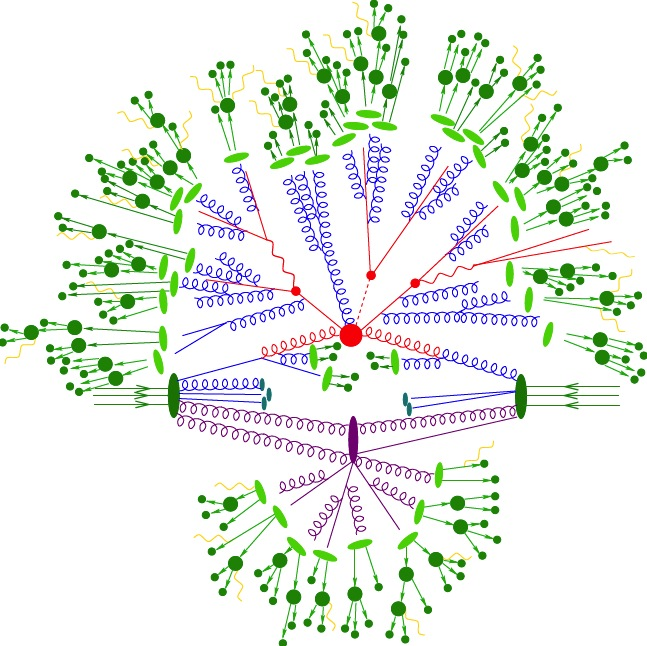
\includegraphics[width=0.6\textwidth]{fig/chapt4/event_sim.jpeg}
%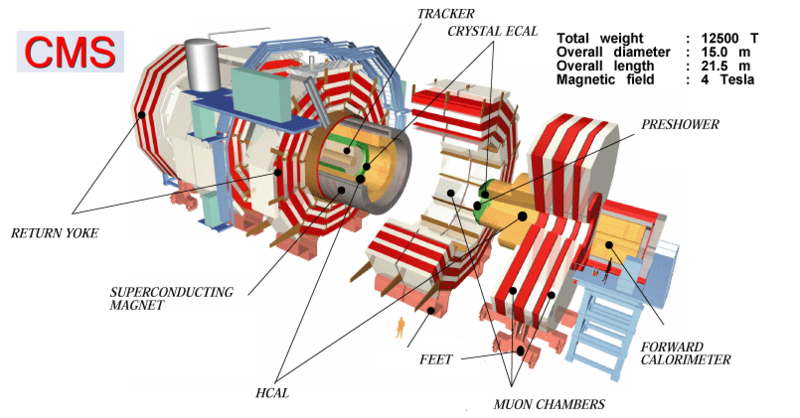
\includegraphics[scale=0.4, trim=20 50 60 30,clip]{fig/chapt3/CMS_exper.png}
\caption{\label{fig:event}The pictorial representation of a $pp$ collision event~\cite{simulated_event}. The hard interaction is represented by the big red blob. Additional hard QCD radiation is produced (red) and a secondary interaction takes place (purple blob) before the final-state partons hadronise (light-green blobs) and hadrons decay (dark green blobs). Photon radiation occurs at any stage (yellow)}.
\end{figure}  
\subsection{Parton distribution functions}
In hadron colliders such as the LHC, the colliding particles (protons) have a composite structure consisting of gluons and quarks. In this analysis, the SM $t\bar t$ and the heavy Higgs (H, A) states are produced by the gluon fusion. Therefore, it is necessary to understand the internal structure of proton, described by the \textit{Parton Distributing Functions (PDFs)}. The parton density function $f_{i}(x, Q^2)$ gives the probability of finding a parton (quarks or gluons) of flavour $i$ in the proton, carrying a fraction $x$ of the proton momentum with $Q$ being the energy scale of the hard interaction~\cite{Placakyte:2011az}. An accurate determination of PDFs, and their corresponding uncertainties is obtained from global fits to a variety of data from multiple experiments, such as HERA, Tevatron, and LHC, using the DGLAP evolution equation. These results show that for small values of $Q^2$, a large fraction of the hadron momentum is carried by its valence quarks; whereas at high energies, most of the hadron momentum is carried by the so-called sea partons, i.e. gluons and virtual $q\bar q$ pairs.

This analysis uses the ``\textsc{nnpdf30}” sets provided by the ``\textsc{nnpdf}” collaboration~\cite{nnpdf_sets}. ``\textsc{nnpdf}” uses an unbiased modelling tool, Neural Networks, with trained genetic algorithms to construct a Monte Carlo representation of PDFs and their uncertainties – a probability distribution in a space of functions. As a final user, a set of 100 MC replica has been used to compute PDF-dependent quantities along with their uncertainties. The central value represent the ``best fit'' PDF, while the error members represent variations around the best result. The PDF uncertainties are discussed in detail in Sec.~\ref{subsec_theo_uncer}.



\subsection{Hard scattering}
The actual interaction of two protons occurs when partons from the two colliding protons interact and produce new particles with high $p_{T}$. These events are of keen interest for analysis and are referred to as hard scattering. If the colliding protons merely undergo soft collision, the resultant particles have low $p_{T}$, commonly known as soft scattering. PDFs describe the structure of the proton and contain the initial momentum distribution of the partons involved in the hard interaction. In hadron-hadron (in case of LHC, it is $pp$) collisions, a wide variety of hard scattering cross sections can be calculated using the QCD factorization theorem and weighting the subprocess cross section with the PDFs extracted from deep inelastic scattering~\cite{hard_scatter}. Factorization theorems separate long- and short-distance physics when calculating these cross sections.   
\begin{equation}\label{eq:xsec}
\sigma_{AB} = \int dx_{a}dx_{b}f_{a/A}(x_{a},\alpha_{s},\mu_{F}).f_{b/B}(x_{b},\alpha_{s},\mu_{F}).\hat{\sigma}(\hat{s};\alpha_{s},\mu_{F},\mu_{R})
\end{equation}  
Where, $f_{a/A}$ is the probability that a parton $a$ inside a hadron $A$ carries a momentum fraction $x_{a}$, $\hat{s}$ is the parton centre-of-mass energy, $\alpha_{s}$ is the strong coupling constant, $\mu_{F}$ is the factorization, and $\mu_{R}$ is the renormalization scale.

\subsection{Particle physics generators}\label{sec:gnerators}
In the current High Energy Physics (HEP) regime, the most challenging aspect is the multiparticle production, where the observed particle multiplicities extend to hundred. These multiplicities are expected to go upward in future HEP colliders. Event Generators (EG), based on computer programs, solve this problem by generating events as detailed as could be observed by a perfect detector.   
In High Energy Physics, a number of Monte Carlo (MC) generators are available to calculate the tree-level diagrams numerically and integrate them over the relevant phase space. A list of them are used in Monte Carlo production for this analysis is discussed below.
\begin{itemize}
\item\textsc{MadGraph:} now merged into \textsc{Mg\_amc@nlo}, a general-purpose event generator~\cite{madgraph} used for the generation of signal samples in this analysis. It is a pure-matrix element generator that generates hadron-hadron ($pp, p\bar{p}, gg, q\bar{q}$) collision and in practice, produces eight particles (quarks, gluons, and leptons) in the final state without hadronization. It also provides an opportunity to produce samples using the interference effect. The interference comes into play when the signal and background have the same final state particles; in this analysis, the signal $gg\rightarrow H/A \rightarrow t\bar{t}$ and the SM $t\bar{t}$, the main background, have same final state particles. 
\textsc{MadGraph} is further interfaced with \textsc{Pythia} or \textsc{Herwig} to generate showering and hadronization steps. The double counting in the showering is solved by applying the MLM scheme. To describe the parton structure, ``\textsc{nnpdf30}'' PDF~\cite{pdf_sets} sets are used in this analysis. 

\item{\textsc{Pythia:}}\label{subsec:pythia} is a multipurpose event generator used frequently in HEP. It provides the possibility to generate complete events in as much detail as experimentally observable within the bounds of our current understanding of the underlying physics. \textsc{Pythia} is used to model $e^{+}e^{-}$, $ep$ and $pp$ collisions and simulate a large variety (over 300) of hard 2 $\rightarrow$ 2 processes that include SM and many BSM processes up to Leading Order (LO) accuracy. \textsc{Pythia} uses the Lund string model~\cite{lund_string_model} to describe hadronization and external PDFs for hard processes calculations. It uses a $p_{T}$-ordered showering technique for parton showering, where partons are ordered by their transverse momentum ($p_{T}$) and $Q^{2} = p^{2}_{T}$ – the closer the parton is to the vicinity of the hard process, the higher $p_{T}$ is assigned to it. More detail about the \textsc{Pythia} program is given in~\cite{pythia}.

\item{\textsc{Powheg:}} PositiveWeight Hardest Emission Generator is an event generator~\cite{powheg} that provides modelling of the hardest interaction at NLO QCD accuracy and needs to be interfaced with \textsc{Pythia} or \textsc{Herwig} for the parton showering and hadronization. The proton structure is described using the PDF sets \textsc{nnpdf30} for the MC samples generated by \textsc{Powheg}.

\item{\textsc{Mc@nlo:}} is an event generator~\cite{mcanlo} that generates hard emissions using NLO fixed-order QCD calculations with the (N)LL accuracy shower algorithm implemented in \textsc{Herwig}. For showering hadronization and decays, the \textsc{Mc@nlo} has to be interfaced with a general-purpose detector such as \textsc{Herwig} or \textsc{Pythia}. The event generation strategy of the \textsc{Mc@nlo} is a two-step process. In the first step (NLO), the hard-scattering events (un-weighted) are generated with NLO QCD accuracy. In the second step (MC), the resultant events are passed to \textsc{Herwig} for further processing (parton-shower, hadronization, decays) and the final events are weighted. A specific fraction of events (20–30\%) with negative weights are assigned in the matching procedure. The negative weights cancel the positive, leaving 40–60\% positive weighted events. To cope with this situation, a large event sample needs to be generated. The PDF sets used by \textsc{Mc@nlo} are \textsc{nnpdf30}.

\item{\textsc{Herwig:}}\label{subsec:herwig} is a general-purpose event generator~\cite{herwig}, which models hadron-hadron, lepton-lepton, and hadron-lepton collisions at LO. Like \textsc{Pythia}, it provides the description of all subprocesses of an event but uses different approaches and algorithms. The \textsc{Herwig} tool implements an angular order showering, $Q^{2} \sim 1 – \cos\theta$, where $\theta$ is the angle between the parent and emitted parton. \textsc{Herwig} exploits the cluster model for showering.
\end{itemize}
\subsection{Parton showering}
The previous section illustrates the generation of a hard process according to lowest-order matrix elements, which results in a limited number of partons in the final state. These describe the momenta of the outgoing jets well, but any fixed order is insufficient to provide a complete picture of the overall process, including the internal structure of the jets and the distribution of the accompanying particles. The effect of all higher-order corrections, including additional ISR/FSR from the branching of the partons, can be simulated through the parton-shower (PS) algorithm. It describes the evolution in momentum transfer from the high-energy scales associated with the hard process down to the low scales of order 1\,GeV associated with the confinement of the partons it describes into hadrons~\cite{parton_shower}. Multi-purpose event generators, like \textsc{Pythia}~\ref{subsec:pythia} and \textsc{Herwig}~\ref{subsec:herwig}, use parton showering algorithms with different implementations. Hard processes can be described well using matrix element calculations, where the partons are energetic and widely separated. It also incorporates the interference effects of amplitudes with the same final state topology. In this work, we produce the interference effect between the signal ($gg\rightarrow H/A\rightarrow t\bar{t}$) and SM $t\bar{t}$ ($gg\rightarrow t\bar{t}$) background using the \textsc{MadGraph} generator defined in Sec.~\ref{sec:gnerators}. The matrix element and parton shower algorithms can be combined to fully describe an event with extra care to avoid double counting in the overlapping phase-space. Different schemes are used for this purpose. CMS uses the MLM algorithm for matching interfaces \textsc{MadGraph} with \textsc{Pythia}, which vetoes the emission of partons by showering above a user-defined matching threshold~\cite{matching}.  
%---------------------------------------
\subsection{Hadronization}
The hadronization process starts after showering, where a set of coloured partons is transformed into a set of colour-singlet primary hadrons, which may decay further to secondary hadrons. Different models are used to describe the fragmentation of the partons after showering. The most commonly used one is the $Lund$ $String$ $Fragmentation$ $Model$, implemented in \textsc{Pythia} and proposed to be universal, i.e. process independent. It is based on the observation that the colour potential of the sources, such as a heavy quark–antiquark pair, increases linearly with their separation~\cite{Mena:2018zyu}. The potential energy increases with the separation of quark–antiquark, and at an order of 1\,fm, it collapses into colour-field strings between them. The original quark pair is now converted into two pairs of quark and antiquark $q\bar{q}\rightarrow q\bar{q}^{'} + q^{'}\bar{q}$; this process continues until only the hadrons remain~\cite{hadronization}. Apart from the hard interaction, other constituents of the colliding proton can also interact, adding additional hadrons in the final state. This is usually referred to as the underlying event (UE) described by special tunes in the generators, such as \textsc{Pythia} uses \textsc{Cuetp8m2t4} in this analysis. During one bunch crossing, the average pp interaction goes up to 35, known as the pile-up, resulting in a relatively low number of $p_{T}$ particles, which can, however, obscure the interesting hard process.
%---------------------------------------
\subsection{Event simulation}
The newly generated particles from the event generator are passed through a chain of processes to simulate the detector's material and magnetic field effects.  
CMS uses two types of MC event simulations – fast simulation (``FastSim'') and full simulation (``FullSim'') – based on the analysis requirement. The ``FastSim'' method reduces the CPU overhead time and is much faster as compared to ``FullSim''. However, it uses a parametric approach to simulate and reconstruct events with the CMS detector and can be used for conducting specific analyses. The alternative ``FullSim'' approach is rather time consuming but more accurate and is based on \textsc{GEANT4}-based simulation~\cite{Agostinelli:2002hh}. The analysis included in this thesis benefits from the ``FullSim'' approach. \textsc{GEANT4} is a toolkit that provides a comprehensive set of physics processes to model the interactions of particles with the detector materials, the resulting energy loss, and the detector’s electronic response. The algorithm incorporates information concerning the material budget, strength of the magnetic field, and the precise geometry of the CMS detector. 

Pile-up events are also added at this stage, which are mostly soft QCD processes. They are simulated as minimum-bias beforehand in the form of a library and then used to overlay onto the signal event according to a specified pile-up scenario. ``Out-of-time'' pile-up information is also taken into account, where many bunch crossings take place before and after the central collision event. 

Digitization is the next step in which information from the previous steps are converted into electronic signals including electronic noise. The L1 and HLT information is also included in the simulated MC samples. The simulated sample's format at this level is similar to that of the real collision data and can pass the same reconstruction steps as the real collision data explained in Sec.~\ref{sec_recons}.  
%------------------------------

\section{Event reconstruction}\label{sec_recons}
The CMS event reconstruction procedure is interpreting the detector data as a set of physical objects, electrons, muons, photons, charged hadrons, and neutral hadrons. In this analysis, the final state objects of the $t\bar t$ system are generally reconstructed using the Particle Flow (PF) algorithm~\cite{Beaudette:2014cea}. This provides a fully consistent picture of the event by reconstructing the particles and jets by taking information from all subdetectors of the CMS. It iterates the event to reconstruct particles and jets, starting from identifying the muons, as they have the most unambiguous particles. After identification, the muon signal is blinded and the charged hadrons are reconstructed. The electron is reconstructed in the next step while the remaining signals in the ECAL are assigned to the photons and the signals from HCAL to the neutral hadrons. Once all the particles and jets have been reconstructed in the event, the missing transverse energy ($E_T^{miss}$) is reconstructed on the basis of all the available information. PF algorithm is applied to data and simulation in the same manner, which generally leads to a good agreement between the data and MC. Sometimes, the quantities are not well modelled in simulation and are further corrected by applying event reweighting techniques to simulation only without hiding the new physics.   
\subsection{Track and vertex reconstruction}
Combinatorial Track Finder (CTF)~\cite{Chatrchyan:2014fea} is used in the CMS experiment as a tracking algorithm – an extension of the Kalman filter~\cite{Fruhwirth:1987fm}.
From the inner tracking detectors, the neighbouring pixels and strips that produce signals are grouped to clusters, which provides the estimate hit of a passing particle from the detector material. A sequence of hits can be used for fitting in order to find the corresponding trajectory of the passing particle. A charged particle is bent inside the magnetic field, producing a curvature that determines the momentum of the particle. Four main steps are involved in track reconstruction.
\begin{itemize}
\item{\textbf{Seed generation:}}
provides initial track candidates using 2–3 tracker hits.
\item{\textbf{Track finding:}}
the seed trajectory is extrapolated to the outer layers of the tracker along the expected flight paths, and further hits that are compatible with the original track are found. On each consecutive layer, all hits from a 3$\sigma$ region around the seed trajectory are tried out and fitted with a Kalman filter.
\item{\textbf{Track fitting:}}
the final collection of hits found in all the tracker layers with the track findings; a track candidate is refitted using the Kalman filter.
\item{\textbf{Track selection:}}
checks if the track candidates satisfy a set of track-quality requirements.
\end{itemize} 
The tracking procedure is repeated six times. On the first iteration, high $p_T$ of the tracks and the smallest impact parameters are required. The tracks reconstructed in the first iteration are blinded, and the second iteration starts with slightly softer requirements
on the seed tracks.
\subsection{Primary vertex reconstruction}
The primary vertex is the location of a proton-proton interaction in the CMS geometrical centre, which is determined separately for each event. The primary vertex reconstruction exploits information from the beam spot, which is the 3D-luminous region inside the CMS detector at the collision point. Its position is considered to be the average of collision points from many events.
The primary vertex reconstruction procedure follows three steps~\cite{Chatrchyan:2014fea}:
\begin{itemize}
\item\textbf{Track selection:}
select tracks that are consistent with being produced in the primary interaction region, having hits in at least two-pixel layers and at least five pixel and strip layers associated with the track and having a $\chi^{2}$ per degree of freedom for the track fit not higher than 20.
\item{\textbf{Track clustering:}}
the clustering algorithm prohibits the tracks from splitting into two and emerging from a single vertex while simultaneously not allowing tracks from different vertices to merge into a single track. The tracks are clustered according to their z-coordinate at the point of closest approach to the beam spot centre.
\item{\textbf{Fitting the vertex position:}}
tracks selected in the previous two steps are used for the fitting using the adaptive vertex filter~\cite{0954-3899-34-12-N01}.
\end{itemize}

The information from all primary vertices in the event is useful for the reconstruction of other objects as well as for separating the signal vertex with a hard interaction from one with a soft interaction. On average, 20 primary vertices can be reconstructed in one event, called a pile-up , corresponding to 20 pp interactions.
\section{Physics objects reconstruction}
The work presented in this thesis exploits the final state of the $t\bar t$ system that consists of leptons (electron, muon), jets, and b-jets originating from b-quarks and missing transverse energy. Their reconstructions in the CMS detector are described below. 
\subsection{Muon reconstruction} 
Compared to other physics objects that mostly stop in the calorimeters or magnet bulk, muons can be identified unambiguously as they travel through the entire detector. A muon can be reconstructed by combining the information from the inner tracking system with that of the muon spectrometers~\cite{Chatrchyan:2012xi}. Muon reconstruction approaches used in CMS analyses follow three methods.
\begin{itemize}
\item\textbf{Standalone muon reconstruction:}
relies only on the muon system; the Kalman filter (KF) fit is performed starting from the track segments in the innermost muon chambers. It is mainly used for the cosmic muon reconstruction because of the large volume of the muon spectrometer. For $pp$ collision, the tracker information is added to increase the precision. 
\item\textbf{Global muon reconstruction:}
muon tracks reconstructed from the muon system only (standalone muon) are fitted together with compatible tracks from the inner tracker using the Kalman filter technique. 
\item\textbf{Tracker muon reconstruction:}
a tracker muon corresponds to a tracker track extrapolated to the muon detector region that is compatible with the position of at least one segment in the muon chambers.
At a lower momentum, $p_T < 5$\,GeV, the tracker muon reconstruction is more efficient; at higher energies, the global muon shows more efficiency. In Fig.~\ref{fig:cms_quadrant}, a schematic view of the transverse plane of the CMS detector is shown with all detectable particles.  
\end{itemize}
The work presented in this thesis uses a global muon reconstructed with the help of the Particle Flow (PF) algorithm. It also reconstructs a non-isolated muon within the jet cone, which is further vetoed during the final event selection. The detailed selection criteria for a tight muon and to veto a loose muon in an event will be described in Sec.~\ref{sebsec:muon_selection}. 
\begin{figure}[h]
\centering
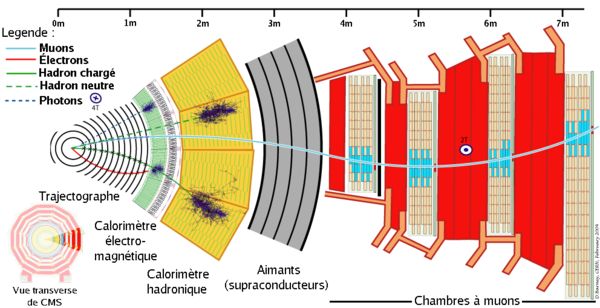
\includegraphics[width=0.7\textwidth]{fig/chapt4/cms_quadrant.png}
\caption{\label{fig:cms_quadrant} A sketch of the particle interactions in a transverse slice of the CMS detector, from the beam interaction region to the muon detector.}
\end{figure}  


\subsection{Electron reconstruction}
Electron reconstruction~\cite{Khachatryan:2015hwa} begins with the clustering of ECAL energy deposits. In the absence of material interactions in the beam pipe or tracker, approximately 94\% of the incident energy of a single electron is contained in 3 × 3 crystals and 97\% in $5\times 5$ crystals. Due to the strong magnetic field and the electrons undergoing Bremsstahlung, the energy deposited in the ECAL is spread in $\phi$. This energy is clustered by building a group of clusters, a supercluster (SC), which is extended in $\phi$. CMS employs a hybrid algorithm in the EB and an island algorithm in the EE.

Non-overlapping clusters are grouped into an SC. The procedure is seeded by searching for the most energetic cluster (seed cluster) and then by collecting other clusters in a fixed search area around the seed position. The clusters belonging to radiation from a single electron are aligned in $\eta$ but spread in $\phi$. By collecting all clusters in a narrow $\eta$ window, whose size is dictated by the $\eta$ resolution of the detector, it is possible to recover most of the radiated energy. The energy of the SC is corrected based on the number of crystals present in the seed cluster in order to remove any residual $\eta$ dependence. The position of the shower is obtained by calculating the energy-weighted mean position of the crystals in the SC [2]. To complete the process of electron reconstruction, the SC needs to be associated with a track in the inner tracker. Electron tracking begins with the formation of a pixel seed, which involves finding a pair of hits in the inner tracker consistent with the trajectory of the electron. The pixel seed itself is a vector located at the outer hit position, pointing in the direction of the electron’s trajectory, and serves as the starting point for tracking. The standard seed-finding process is referred to as pixel-matching since the hit pair is usually located in the pixel layers.

However, a major difficulty of electron reconstruction is that electrons can undergo bremsstrahlung in the tracker material. The radiation affects both energy and momentum measurements, and this effect depends on the material thickness. To account for bremsstrahlung losses, CMS employs a Gaussian-Sum Filter (GSF) track fit. This fit uses the Bethe-Heitler model of electron energy loss and approximates the energy loss distribution as a sum of Gaussian distributions. Different Gaussian models have different degrees of hardness of the bremsstrahlung in the layer under consideration. The GSF fit allows for good momentum resolution at the vertex while also providing a meaningful estimate of the momentum at the outermost part of the tracker.

Largely, there are four types of electron candidates – prompt, non-prompt, conversion, and fake. Prompt electrons are mainly formed by the decay of W and Z bosons. Non-prompt electrons arise from b or c quarks decaying to an electron. Although these electrons are usually not isolated within the quark jet, since there is a significant amount of nearby electromagnetic and/or hadronic activity, the kick from the quark decay might knock the electron out of the jet, enough for it to appear isolated. Conversion electrons come from a photon producing an electron-positron pair in the tracker. Fake electrons are a result of reconstruction error – a coincidence of a jet depositing a large amount of energy in the ECAL and a nearby (matched) single; high-$p_T$ track is misinterpreted as an electron. 

The electron used in this analysis is a PF candidate, passes trigger selection as explained in Sec.~\ref{subsec:elec_trigg}, and uses cut-based identification (ID) recommended for 2016 data samples with different selection criteria for barrel and endcap regions~\cite{Wiki:ElectronID}. The selection criterion further uses tight and loose cuts according to the analysis requirements, as explained in Sec.~\ref{subsec:electron}. 

\subsection{Jet reconstruction}
Jets containing cascades of hadrons, electrons, and photons are clustered to determine the original quark or gluon characteristics. The CMS particle-flow jet identification criteria~\cite{CMS-PAS-PFT-10-002} are used for the jets. This approach uses a jet-clustering algorithm to identify and cluster jets. In the CMS experiment, jets are clustered using anti-$k_T$ clustering algorithm~\cite{Cacciari:2008gp}. Particles with energy above a certain threshold are reconstructed using the PF algorithm within a jet cone size "$\Delta R$" of 0.5. All PF jets below 10\,GeV are considered to represent uncluttered energy. Jet energy corrections that include offset (L1FastJet with an active area calculation), relative (L2), and absolute (L3) are applied. The purpose of the offset term is to correct for the pile-up. The relative corrections smooth out any $\eta$ dependence, and the absolute corrections relate to the overall energy scale. Additionally, jets in data have residual corrections applied to them in order to account for data-Monte Carlo simulation discrepancies. Jets are selected with $p_T >$ 20\,GeV and $\abs{\eta} <$ 2.4 and are further required to satisfy loose quality criteria that suppresses noise and spurious energy deposits:
\begin{itemize}
\item {at least two particles (with at least one being charged in a given jet);}
\item {energy fraction of neutral hadrons < 0.99;}
\item {contribution of both charged and neutral electromagnetic energy fractions < 0.99.}
\end{itemize}
Typical jet energy fractions carried by charged particles, photons, and neutral hadrons are 65\%, 25\%, and 10\%, respectively. This means that 90\% of the jet energy can be reconstructed quite precisely, both in magnitude and direction, by the PF algorithm; the remaining 10\% fraction of energy of neutral hadrons is affected by the poor HCAL resolution and by calibration corrections of about 10 to 20\% (a source of uncertainty that ECAL does not suffer from). Consequently, jets made of reconstructed particles are much closer to jets made of generated particles than jets reconstructed using only calorimeter information with respect to energy, direction, and content.
%-------------------
\subsection{Heavy flavour jet identification}
The accurate identification of heavy flavour jets is important for many searches concerning the LHC (top quark, Higgs boson, and SUSY), which includes light and heavy jets as final state objects. This thesis is based on the $t\bar t$ semileptonic final state search that contains at least four jets with two heavy flavour bjets and two light jets. bjets arise from b quark radiation and hadronization and are identified with the help of different algorithms, commonly known as b-tagging. B-tagging algorithms use variables connected to the properties of heavy-flavour hadrons, e.g. the lifetime of hadrons containing b quarks is more than that of those with c quarks; hence, it decays after covering a few mm to 1\,cm distance, making a displaced secondary vertex (SV). The left Fig.~\ref{Fig:heavy_flavour} shows the displaced SV originated from the decay of a heavy flavour jet. b-tagging algorithms exploit the impact parameter (IP) that characterizes the distance between the primary vertex and the displaced tracks at their points of closest approach. The algorithms further benefit from other measurable quantities, such as the masses of heavy hadrons and the presence of charged leptons in their decay. 

During Run-I, CMS had been using the jet probability (JP) and combined secondary vertex (CSV) taggers; in Run-II, the CSV is optimized to CSVv2 and another version (DeepCSV) is introduced~\cite{Sirunyan:2017ezt}. A new tagger cMVA is introduced in Run-II, based on the combined multivariate analysis, that combines the discriminator values of various taggers. We use cMVAv2 tagger at a medium value (cMVAv2 > 0.4432) with a b-tagging efficiency of about 70\%. The right plot in Fig.~\ref{Fig:heavy_flavour} is the cMVAv2 distribution in data and MC. The medium value (cMVAv2 > 0.4432) clearly selects the region (red color) with high bjets efficiency. A detailed description of the cMVA application in this analysis is given in Sec.~\ref{Sec:BTagReweighting}.    

\begin{figure}
 \centering
 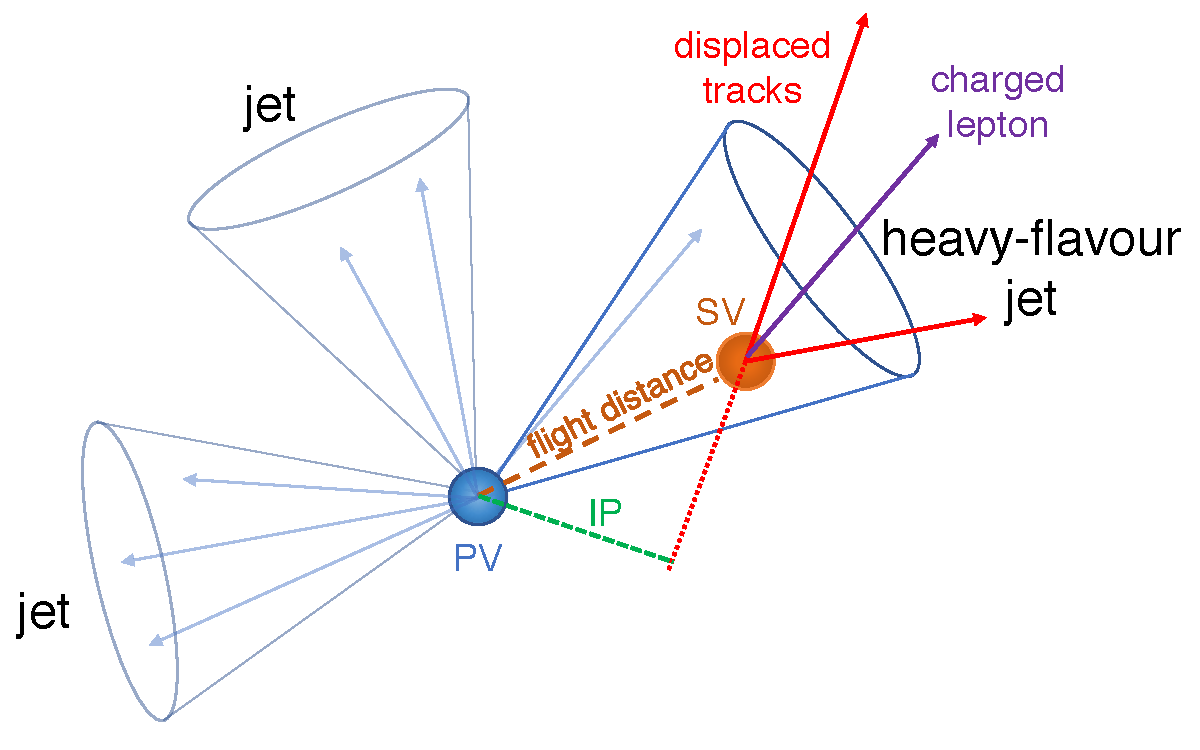
\includegraphics[width=0.47\textwidth]{fig/chapt4/b_jets/secondary_vertex.pdf}\qquad
 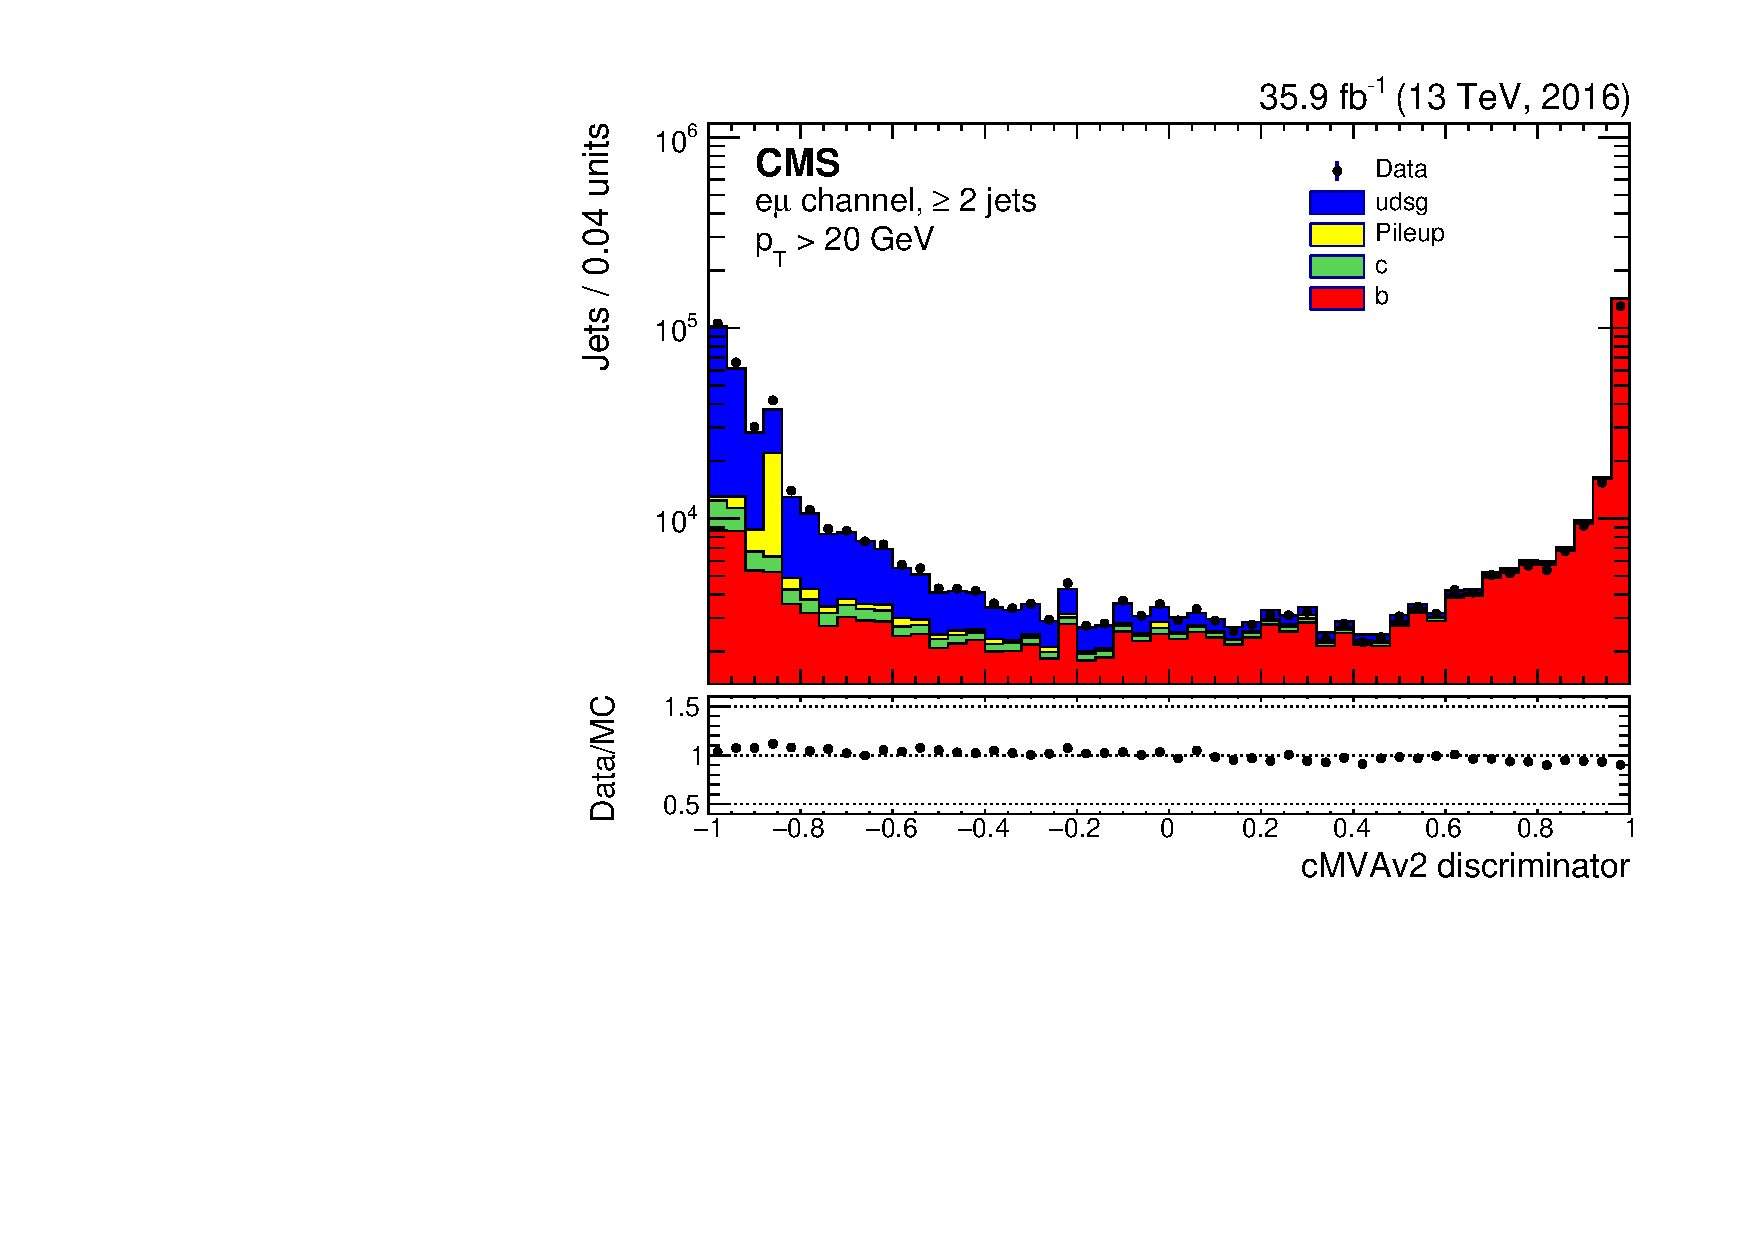
\includegraphics[width=0.47\textwidth]{fig/chapt4/b_jets/cMVAv2.pdf}
 \caption{Left: A heavy-flavour jet ($b/c$) decays from a secondary vertex (SV) resulting in charged-particle tracks (including possibly a soft lepton) with a large impact parameter (IP) value.  Right: The cMVAv2 distribution in data and MC.}
 \label{Fig:heavy_flavour}
\end{figure}
%-------------------
\subsection{Missing transverse energy}
The $E_{T}^{miss}$ can be defined as the imbalance in the transverse momentum of all particles that interact with detectors in an event. Owing to the momentum conservation, $E_{T}^{miss}$ corresponds to the transverse momentum that is carried by weakly interacting particles, such as neutrinos. The $E_{T}^{miss}$ is computed as the negative of the vectorial sum of transverse momenta of all PF particles and is also referred to as PF $E_{T}^{miss}$. This quantity is used in a majority of CMS analyses because of its high performance. 
Minimum energy thresholds in the calorimeters, inefficiencies in the tracker, and nonlinearity of the response of the calorimeter for hadronic particles could lead to overestimated or underestimated values of $E_{T}^{miss}$.

\section{Signal modelling}\label{Sec:SgnModelling}
Assuming that the sought-after heavy Higgs boson respects the usual hierarchy of couplings to fermions, its dominant production mode is the gluon fusion, as shown in Fig.~\ref{Fig:FeynDiagrams} (left).
Only the contribution with the top quark running in the loop is considered, while the subleading term with the bottom quark is neglected as $m_{b} \ll m_{t}$.
The neglected contribution can become significant in models that enhance the coupling to bottom quarks and suppress the coupling to top quarks, such as type-II 2HDM in case of a large $\tan\beta$ value.
Such models are not addressed in this study as they would also decrease the $\Phi \rightarrow t\bar t$ branching ratio.

The squared amplitude corresponding to the signal diagram gives rise to a resonant excess above the SM $gg \rightarrow t\bar t$ production, an example diagram for which is given in Fig.~\ref{Fig:FeynDiagrams} (right).
As with other BSM $t\bar t$~resonances, the excess has an approximately Breit–Wigner $m_{t\bar t}$~spectrum.
Since the signal and the SM processes share the same initial and final states, there is also a contribution from the interference between the two.
The background amplitude is much larger in value than the signal value; because of this, the overall BSM signature can be dominated by the interference.
For the purpose of searching for the new particle, both the resonant Breit–Wigner and the interference are considered as parts of the signal process.

\begin{figure}
 \centering
 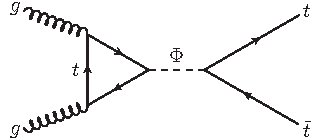
\includegraphics{fig/chapt4/sgn.pdf}\qquad
 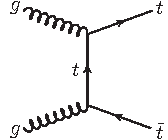
\includegraphics{fig/chapt4/tt-tchan.pdf}
 \caption{Feynman diagram for the signal process (left) and an example diagram for the SM $t\bar t$~production (right).}
 \label{Fig:FeynDiagrams}
\end{figure}
\subsection{Analytical calculation}
%
The leading-order cross section of the $gg \rightarrow t\bar t$ process, with the contribution from the heavy Higgs boson taken into account, was computed in Ref.~\cite{Dicus:1994bm}.
The result obtained there for the $\mathcal{CP}$-even state can be adapted as follows:
\begin{linenomath}
\begin{multline}
 \sigma_H(\hat{s}) - \sigma_\text{QCD}(\hat{s}) = g_{Htt}^4 \cdot \frac{3 \alpha_s^2 G_F^2 m_t^6 \beta^3}{1024 \pi^3} \frac{16 + 8\beta^2 \left(\pi^2 - y^2\right) + \beta^4 \left(\pi^2 + y^2\right)^2}{\left(\hat{s} - m_{\Phi}^2\right)^2 + m_{\Phi}^2\Gamma_{\Phi}^2} \\
 - g_{Htt}^2 \cdot \frac{\alpha_s^2 G_F m_t^4 \beta^2 y}{32 \pi \sqrt{2}\,\hat{s}} \frac{\left(\hat{s} - m_{\Phi}^2\right) \left(4 + \beta^2 \left(\pi^2 - y^2\right)\right) + 2 \pi \beta^2 m_\Phi \Gamma_\Phi y}{\left(\hat{s} - m_{\Phi}^2\right)^2 + m_{\Phi}^2\Gamma_{\Phi}^2},
 \label{Eq:XSecCPEven}
\end{multline}
\end{linenomath}
Where $\sqrt{\hat s}$ is the invariant mass of the incoming gluons; $\sigma_\text{QCD}$ is the SM cross section; $\alpha_s$ and $G_F$ are the strong coupling strength and the Fermi constant respectively; $m_t$ is the mass of the top quark; and $m_\Phi$ and $\Gamma_\Phi$ are the mass and the total width of the heavy Higgs boson.
\begin{linenomath}
\begin{equation}
 \beta = \sqrt{1 - \frac{4 m_{t}^2}{\hat{s}}}\quad\text{and}\quad y = \ln\left(\frac{1 + \beta}{1 - \beta}\right)
\end{equation}
\end{linenomath}
can be interpreted, respectively, as the velocity and twice the rapidity of the top quark in the centre-of-mass frame.
For simplicity, the energy-dependent width in Ref.~\cite{Dicus:1994bm} has been replaced by a constant one, effectively adopting the fixed-width scheme.
The cross section for a pseudoscalar particle, obtained in a similar way, is:
\begin{linenomath}
\begin{multline}
 \sigma_A(\hat{s}) - \sigma_\text{QCD}(\hat{s}) = g_{Att}^4 \cdot \frac{3 \alpha_s^2 G_F^2 m_{t}^6 \beta}{1024 \pi^3} \frac{\left(\pi^2 + y^2\right)^2}{\left(\hat{s} - m_{\Phi}^2\right)^2 + m_{\Phi}^2\Gamma_{\Phi}^2} \\
 - g_{Att}^2 \cdot \frac{\alpha_s^2 G_F m_{t}^4 y}{32 \pi \sqrt{2}\,\hat{s}} \frac{\left(\hat{s} - m_{\Phi}^2\right) \left(\pi^2 - y^2\right) + 2 \pi m_\Phi \Gamma_\Phi y}{\left(\hat{s} - m_{\Phi}^2\right)^2 + m_{\Phi}^2\Gamma_{\Phi}^2}.
 \label{Eq:XSecCPOdd}
\end{multline}
\end{linenomath}

The terms proportional to $g^4$ in Eqs.~\ref{Eq:XSecCPEven} and \ref{Eq:XSecCPOdd} correspond to the square of the amplitude given by the signal Feynman diagram in Fig.~\ref{Fig:FeynDiagrams}.
They produce the usual resonant peak in the m$_{t\bar t}$~spectrum.
On the other hand, the interference terms, which are proportional to $g^2$, result in a complex peak–dip structure.
Both contributions, along with their sum, are shown in Fig.~\ref{Fig:AnalyticXSec} for a width $\Gamma_\Phi = 0.1 \cdot m_\Phi$ and in App.~\ref{app2} for other example values.
The coupling scale factor is set to unity in these plots.
As can be seen, the dip tends to dominate the combined line shape for larger masses and widths, which means that in certain cases, the presence of the heavy Higgs boson can manifest itself with a localized deficit in the m$_{t\bar t}$~spectrum.

\begin{figure}
 \centering
 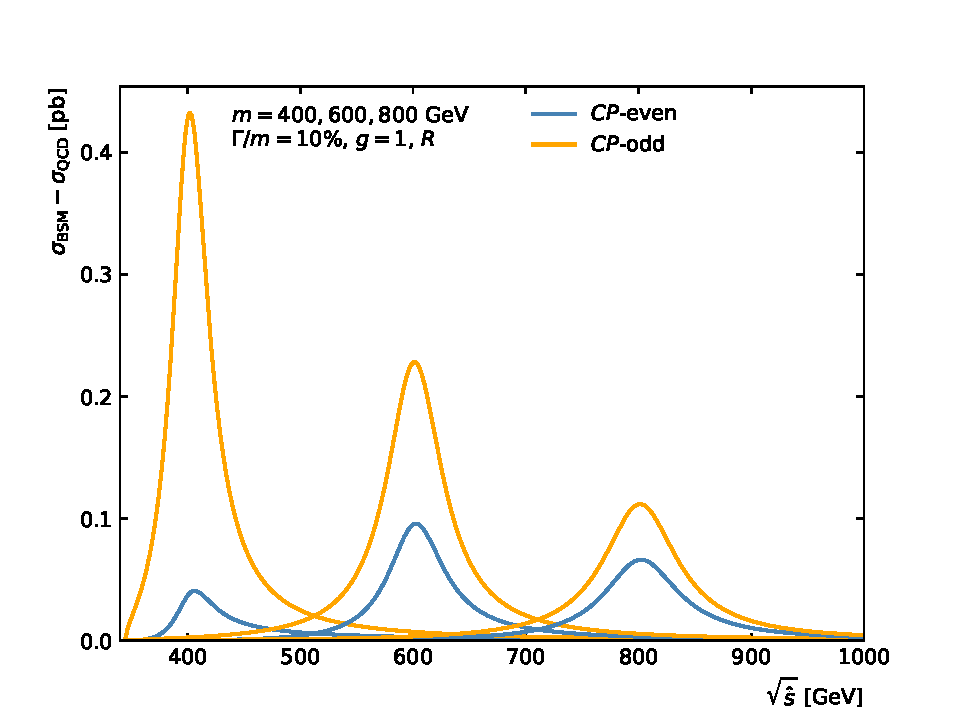
\includegraphics[width=0.49\textwidth]{fig/chapt4/gen_plots/analytical/xSec_relW10_R.pdf}
 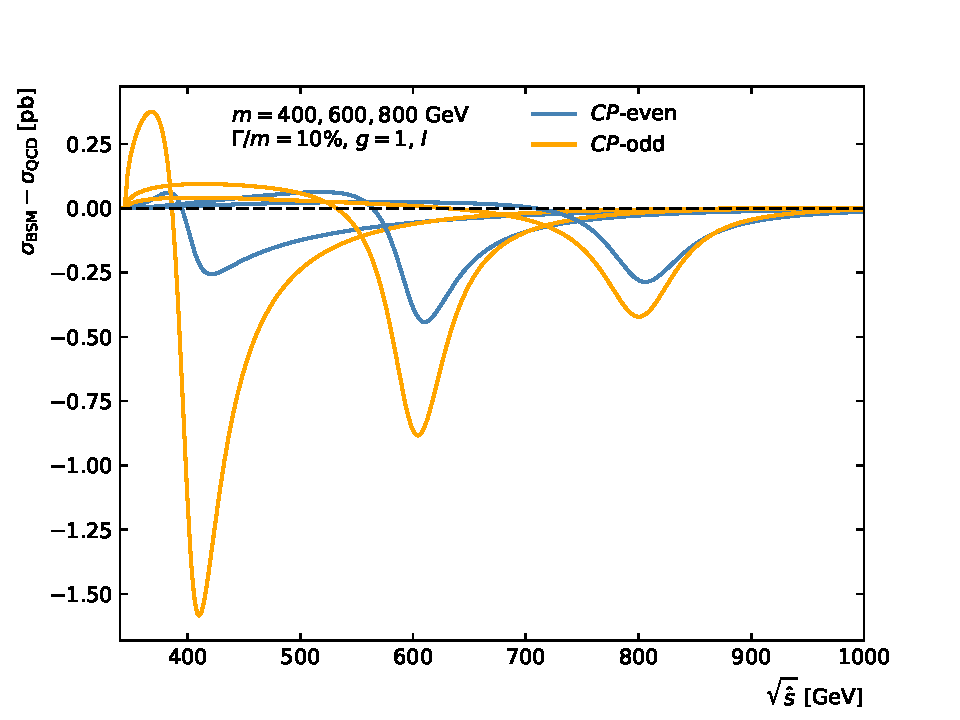
\includegraphics[width=0.49\textwidth]{fig/chapt4/gen_plots/analytical/xSec_relW10_I.pdf} \\
 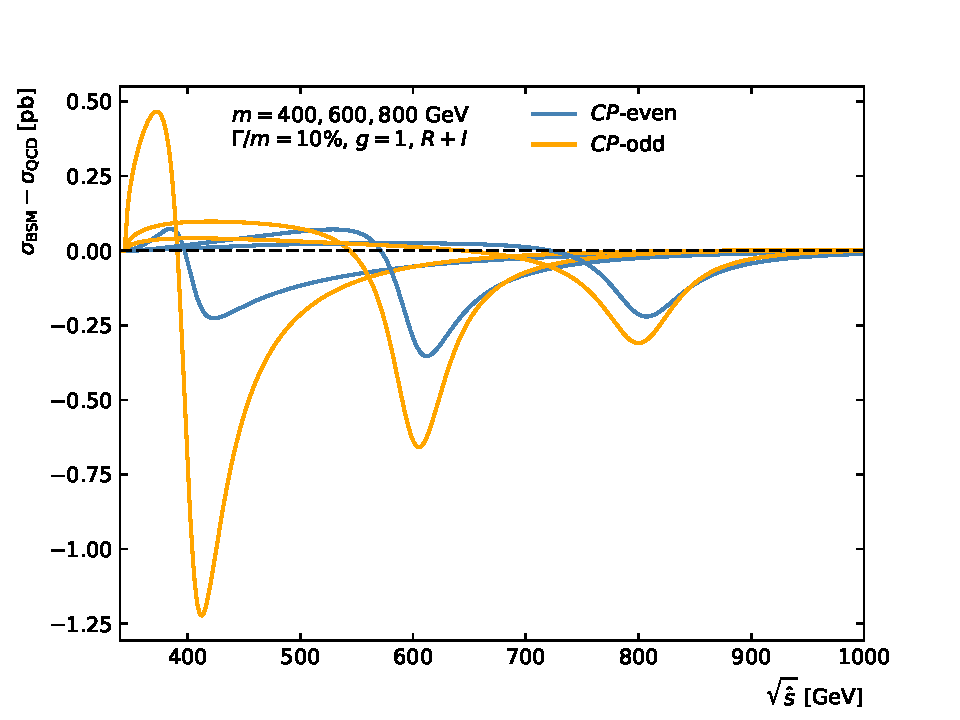
\includegraphics[width=0.49\textwidth]{fig/chapt4/gen_plots/analytical/xSec_relW10_Sum.pdf}
 \caption{Example parton-level cross sections for the resonant part of the signal (upper left), the interference (upper right), and the sum of the two (bottom), with $g = 1$, shown as a function of $\sqrt{\hat{s}} = m_{t\bar t}$. Computed using Eqs.~\ref{Eq:XSecCPEven} and \ref{Eq:XSecCPOdd}. The total width is 10\%.}
 \label{Fig:AnalyticXSec}
\end{figure}

In this search, the heavy Higgs boson is not required to decay exclusively to top quark pairs, which means that its total width is not fixed by the coupling scale factor but only bounded from below with the partial width $\Gamma_{\Phi\rightarrow t\bar t}$.
The latter can be computed for the two $\mathcal{CP}$~states as follows~\cite{Dicus:1994bm}:
\begin{linenomath}
\begin{equation}
\begin{gathered}
 \Gamma_{H\rightarrow t\bar t} = g_{Htt}^2 \frac{3 G_F m_{t}^2 m_\Phi}{4\pi \sqrt{2}} \left(1 - \frac{4 m_{t}^2}{m_\Phi^2}\right)^{3/2}, \\
 \Gamma_{A\rightarrow t\bar t} = g_{Att}^2 \frac{3 G_F m_{t}^2 m_\Phi}{4\pi \sqrt{2}} \left(1 - \frac{4 m_{t}^2}{m_\Phi^2}\right)^{1/2},
\end{gathered}
\label{Eq:Width}
\end{equation}
\end{linenomath}

Where the Higgs boson has been put on the mass shell. The dependence of the partial width on the mass of the particle is shown in Fig.~\ref{fig:Higgs_width}.
For $m_\Phi \gg 2m_{t}$ and $g = 1$ the relative partial width is about 6\%.

\begin{figure}
  \centering
  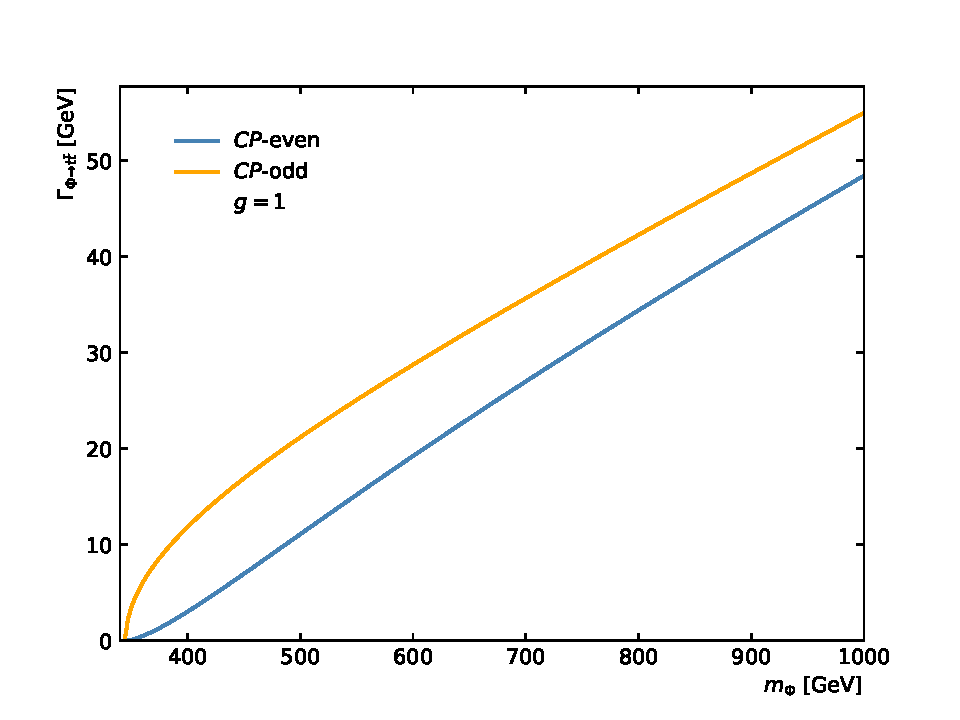
\includegraphics[width=0.6\textwidth]{fig/chapt4/gen_plots/analytical/width.pdf}
  \caption{The partial width of the $\Phi \rightarrow t\bar t$ decay as a function of the mass of the heavy Higgs boson. Computed for $g = 1$.}
  \label{fig:Higgs_width}
\end{figure}

BSM models with an extended Higgs sector typically include additional scalars of each $\mathcal{CP}$~state.
However, there is no interference between the $gg \rightarrow H \rightarrow t\bar t$ and $gg \rightarrow A \rightarrow t\bar t$ processes; therefore, a prediction for the full $gg \rightarrow t\bar t$ production can be constructed in a straightforward manner.
Although this thesis mainly focuses on one $\mathcal{CP}$~state at a time as the main analysis, the combination~\cite{CMS-AN-17-202} is added in chapter~\ref{chapt:8} also considers a case where both states are present.

\subsection{Event generation and validation}
\label{sec:sig_gen_val}
%
Signal events are generated with the $\textsc{MadGraph5\_amc@nlo}$ program~\cite{Alwall:2011uj}, version 2.5.1, which is run in the leading-order mode.
A custom $\textsc{MadGraph}$ model~\cite{MassiveHiggsUFO} adds a heavy Higgs boson to the SM, with the couplings to top quarks defined in Eq.~\ref{Eq:Coupling}.
The effective coupling to gluons is implemented at the leading order following Ref.~\cite{Spira:1995rr}; only top quarks are included in the loop. % Eqs. 67, 53, 54 from the reference.
This model has been cross-checked against the one used in Ref.~\cite{Hespel:2016qaf}.
Following the choice in Ref.~\cite{Hespel:2016qaf}, the factorization and renormalization scales are set on a per-event basis to $m_{t\bar t} / 2$.
The leading-order PDF set \textsc{nnpdf3.0}~\cite{Ball:2014uwa} is used.
The produced top quarks are decayed in $\textsc{MadGraph5\_amc@nlo}$, which preserves spin correlations.
Showering and hadronization are implemented with the $\textsc{Pythia~8}$ program~\cite{Sjostrand:2007gs}, using the tune \textsc{cuetp8m2t4}~\cite{CMS-PAS-TOP-16-021}.
Given that the sought-after particle can only manifest itself in small deviations from the SM $t\bar t$~production, it is impractical to generate the full $gg \rightarrow t\bar t$ process with the BSM contribution.
Instead, only the resonant part and interference are generated, which are then used along with the centrally produced SM~$t\bar t$ sample.
Samples corresponding to the two signal components are created separately.
While event generation for the resonant part poses no technical difficulty; in the case of the interference, the situation is complicated by the fact that $\textsc{MadGraph5\_amc@nlo}$ does not support decay chains with the squared order syntax~\cite{MadGraphIntDecays}, which would be required to keep only interference terms in the squared matrix element.

Production of interference samples involves modification of the Fortran code generated by $\textsc{MadGraph5\_a-}$\\
$\textsc{mc@nlo}$.
Let $C_{\Phi tt}$ be the coupling of the heavy Higgs boson to top quarks, which is utilized by the routine that evaluates the squared matrix element $\abs{\mathcal{M}}^2$.
The code is modified at the point where this routine is called in the following way.
First, $\abs{\mathcal{M}}^2$ is evaluated for the nominal value of $C_{\Phi tt}$ and saved.
Then, the sign of $C_{\Phi tt}$ is flipped, and $\abs{\mathcal{M}}^2$ is computed again, yielding value $\abs{\mathcal{M}(-C_{\Phi tt})}^2$.
The effective coupling of $\Phi$ to gluons is controlled by an independent parameter in the routine and is therefore not affected by the modification of $C_{\Phi tt}$.
As a result, the signs of the interference terms in $\abs{\mathcal{M}}^2$ are flipped, while the SM terms (independent of the $\Phi$~couplings) and the resonant BSM part (proportional to $C_{\Phi tt}^2$) are left unchanged.
Finally, the value $(\mathcal{M}^{2}(C_{\Phi tt}) - \mathcal{M}^{2}(-C_{\Phi tt})) / 2$ is computed and then used in place of the original squared matrix element everywhere.
All terms except the interference terms cancel out in this computation.

The part of $\abs{\mathcal M}^2$ that represents the interference can be written as $2\Re(A_S A_B^\dagger)$, where $A_S$ and $A_B$ are the amplitude of the signal process and the sum of amplitudes for all SM diagrams respectively.
Unlike the usual squared matrix element, this quantity can be negative in some regions of the phase space; this fact is reflected in the sign of event weights assigned by the generator.

The generation procedure is validated for an example of a pseudoscalar particle with a mass of 500\,GeV and 10\% width.
A sample of 40~M events is generated for the full $gg \rightarrow t\bar t$ process.
The interference is then modelled by subtracting the SM-only production (40~M events) and the resonant $\Phi$~production (400~k events) from it, all normalized to the respective leading-order cross sections.
Distributions of various observables are compared between this reference construction and the method described above.
The comparison for the $t\bar t$ invariant mass is shown in Fig.~\ref{fig:GENcomparison_mtt}, and App.~\ref{app3} includes other observables along with additional details about the validation.
Although some small discrepancies can be observed, they are consistent with statistical fluctuations.

\begin{figure}
  \centering
  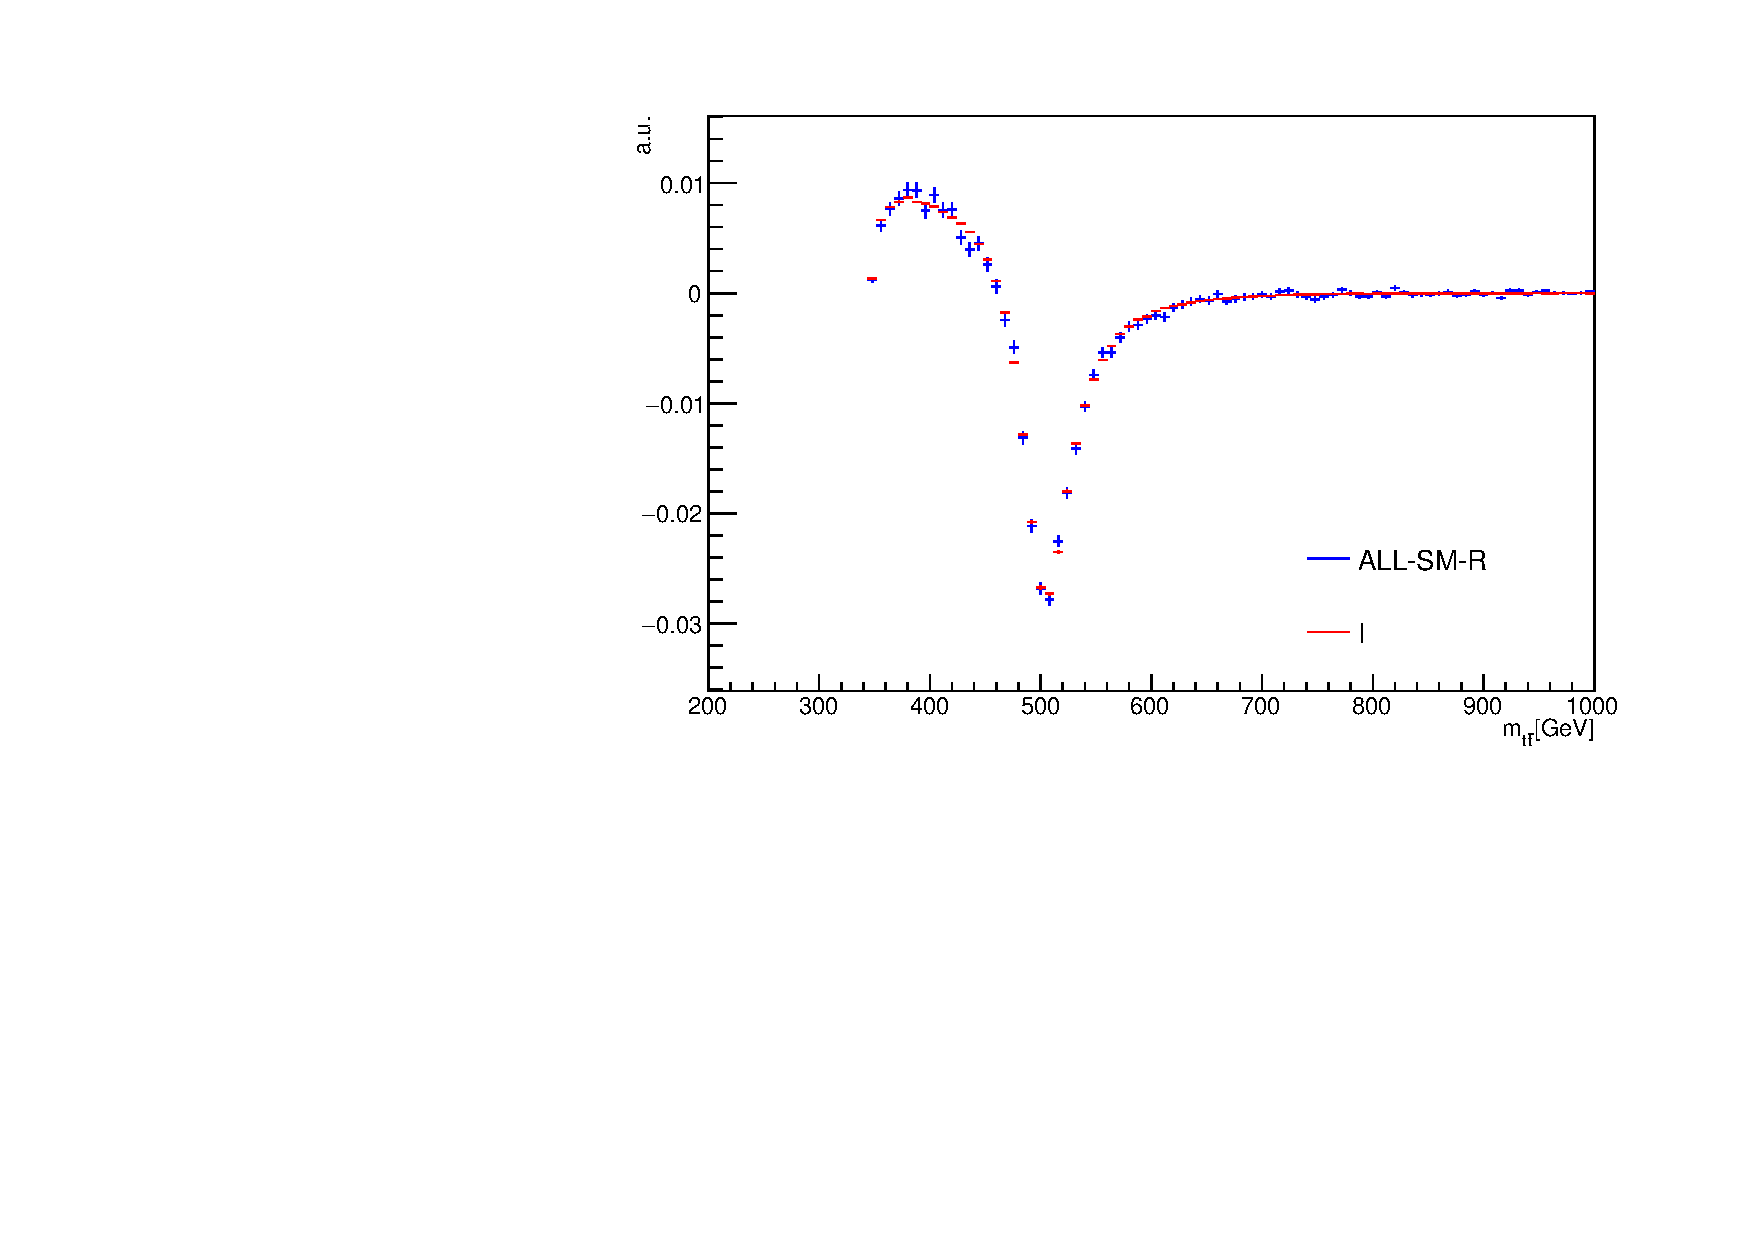
\includegraphics[width=0.6\textwidth]{fig/chapt4/gen_plots/mtt_compare.pdf}
  \caption{Spectra of $m_{tt}$ in the interference obtained by the modification of the generated squared matrix element (red) and the validation procedure detailed in the text (blue).}
  \label{fig:GENcomparison_mtt}
\end{figure}

A number of versions of signal samples have been produced to scan parameters of the heavy Higgs boson.
The couplings $(g_{Htt}, g_{Att})$ are set either to $(1, 0)$ or $(0, 1)$.
This results in pure $\mathcal{CP}$~states, which, as discussed above, can be mixed in a straightforward manner if required.
Since samples for the resonant part and the interference are generated independently, distributions for any values of the coupling can be reproduced by scaling the normalization factors with $g^4$ and $g^2$ respectively (cf. Eqs.~\ref{Eq:XSecCPEven} and \ref{Eq:XSecCPOdd}).
Four mass hypotheses are modelled for each $\mathcal{CP}$~state: 400, 500, 600, and 750\,GeV.
For each mass point, the generation is performed for a total width of 2.5, 5, 10, 25, and 50\%, where the \% is with respect to the mass point. For example, 10\% of mass 500\,GeV is a 50\,GeV width.
Furthermore, samples with the two final states are produced.
In the first group, one of the top quarks must decay, producing an electron or a muon (but not a tau lepton), while the other one must decay to quarks.
In the second group, each of the top quarks must decay, producing a charged lepton of any generation.
These samples are mostly intended for the complementary search in the dilepton channel but nonetheless account for a small fraction of selected events in the $l+jets$ channel.

Figures~\ref{fig:mtt_gen_400} to \ref{fig:mtt_gen_750} show distributions of the $t\bar t$ invariant mass for different signal hypotheses.
The resonant and interference parts are shown separately, all normalized to the same area.
\begin{figure} \centering
  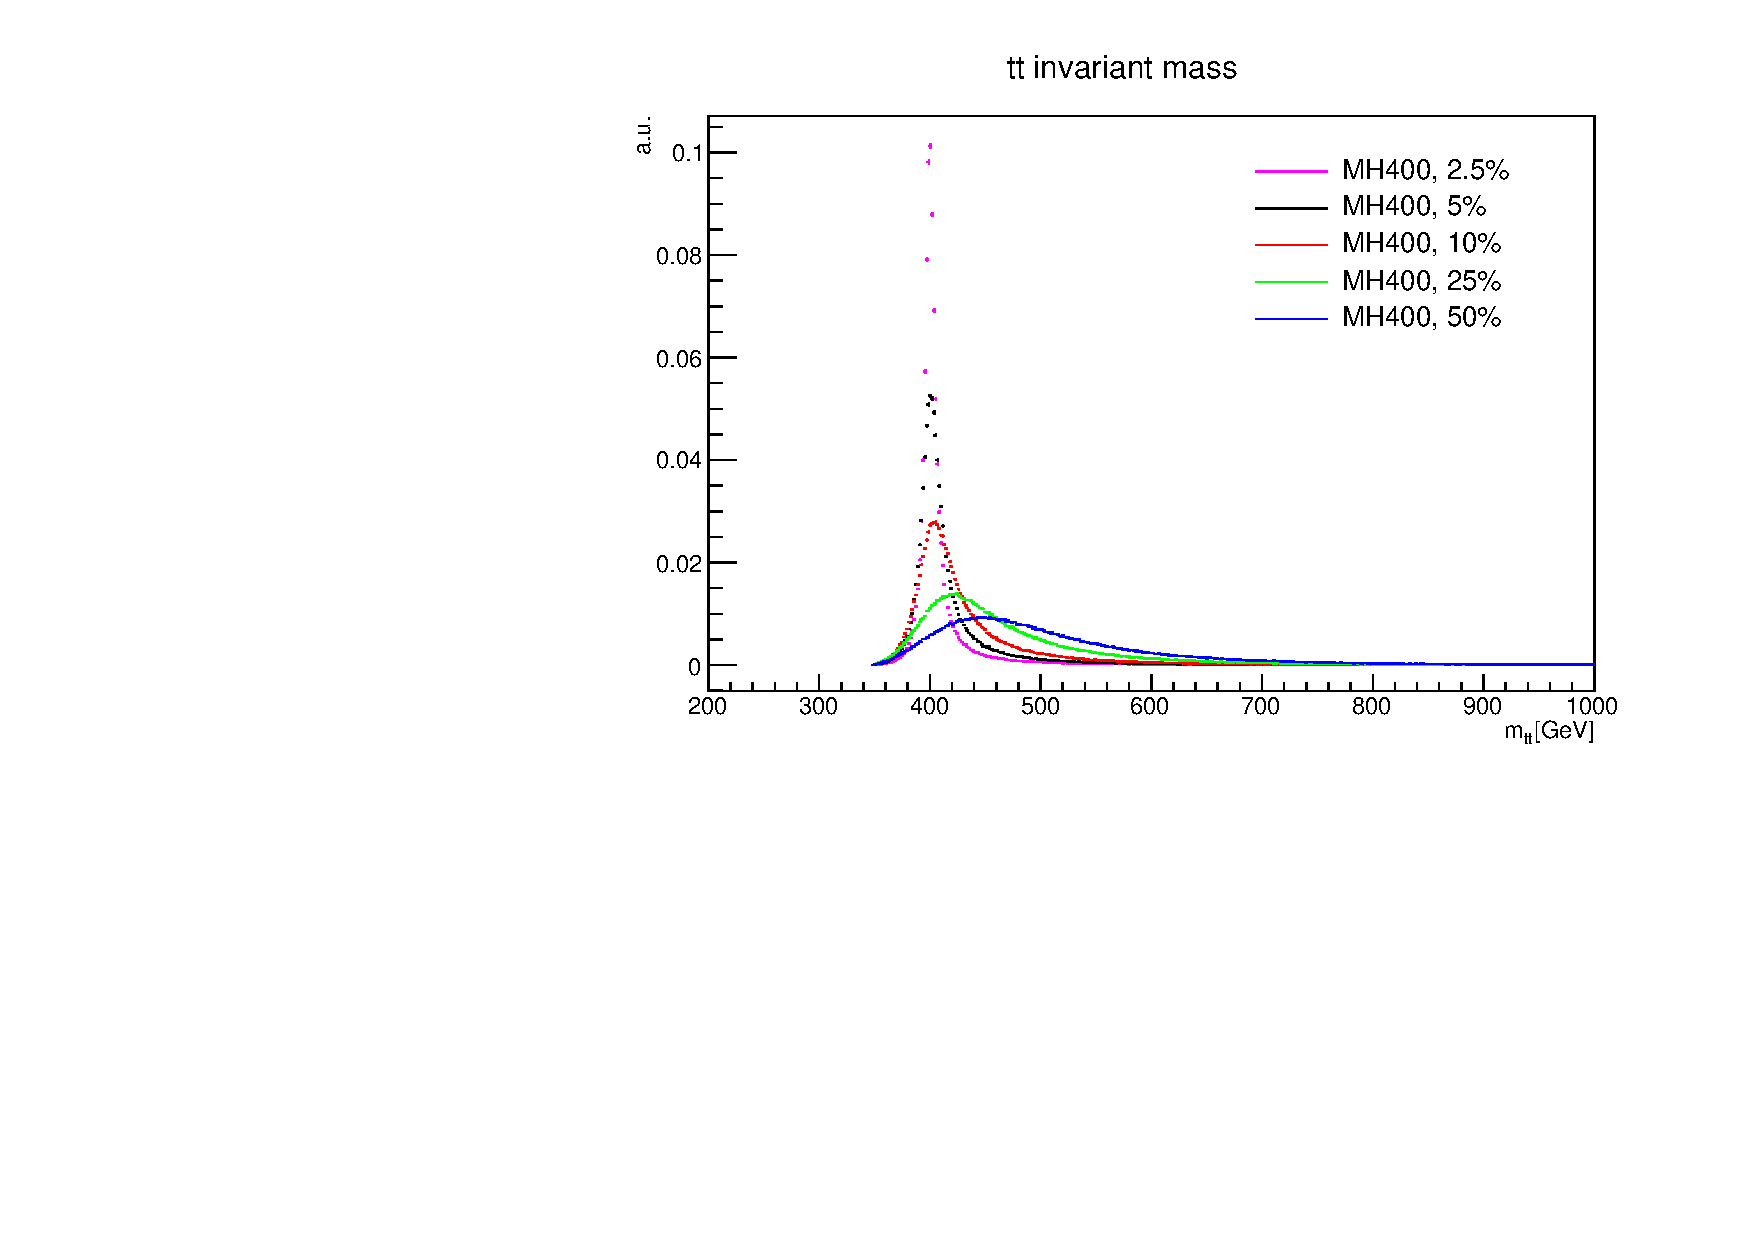
\includegraphics[width=0.4\textwidth]{fig/chapt4/gen_plots/H_res_ljets_M400.pdf}
  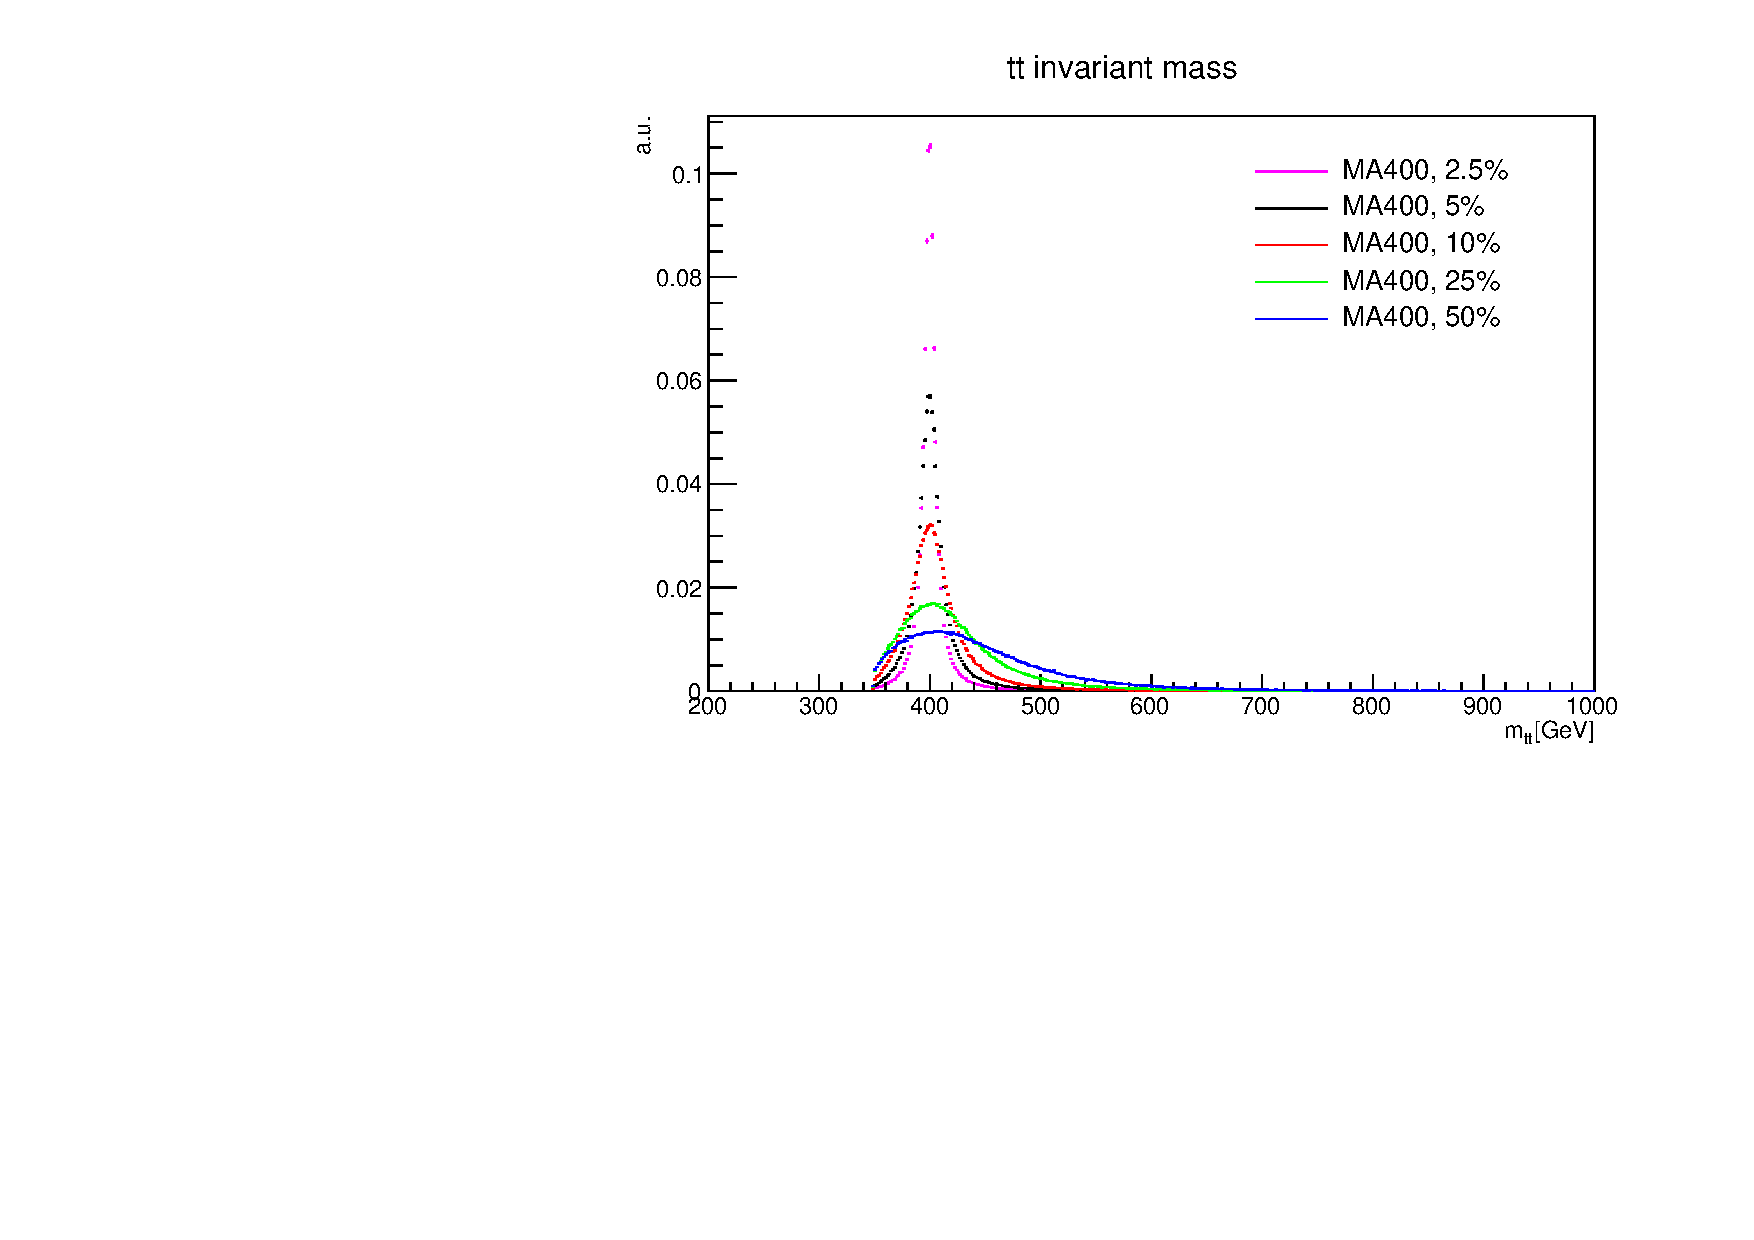
\includegraphics[width=0.4\textwidth]{fig/chapt4/gen_plots/A_res_ljets_M400.pdf}\\
  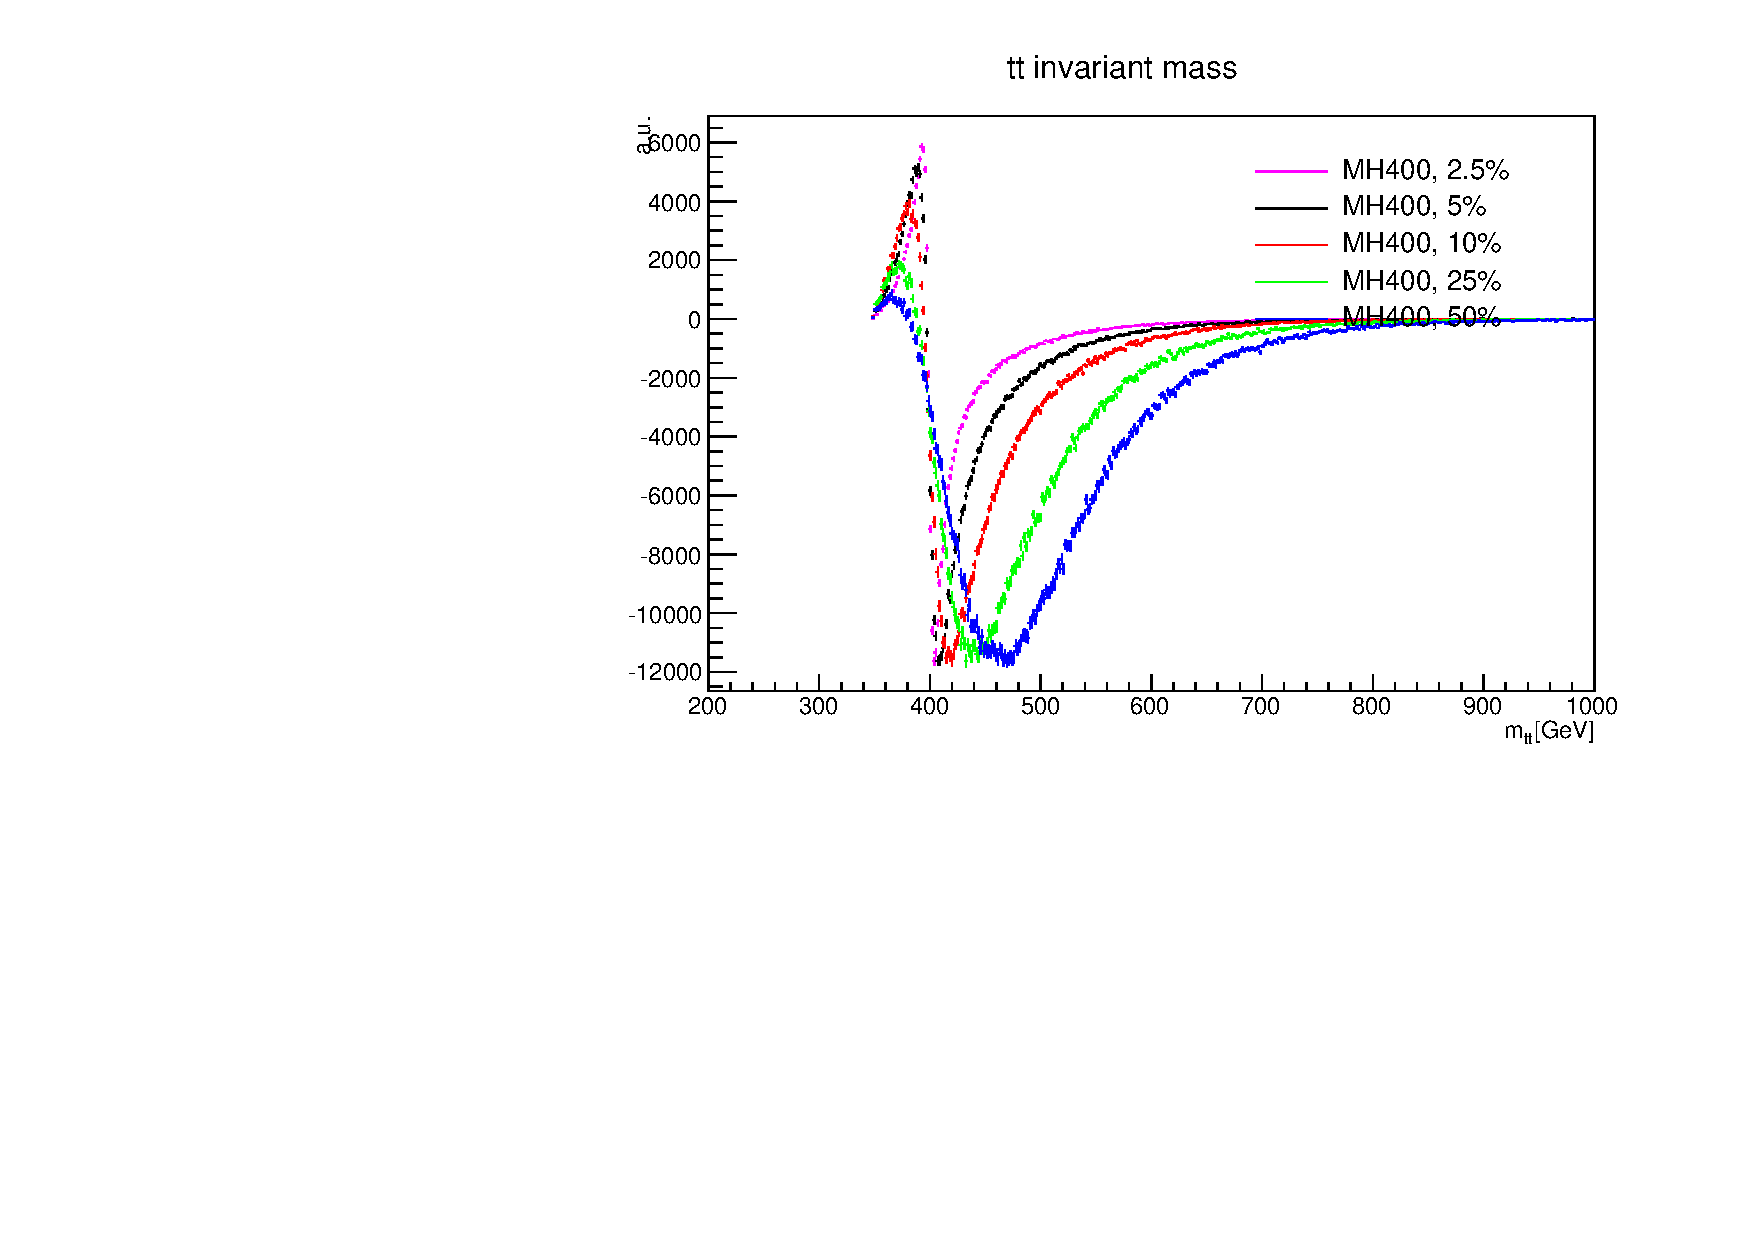
\includegraphics[width=0.4\textwidth]{fig/chapt4/gen_plots/H_int_ljets_M400.pdf}
  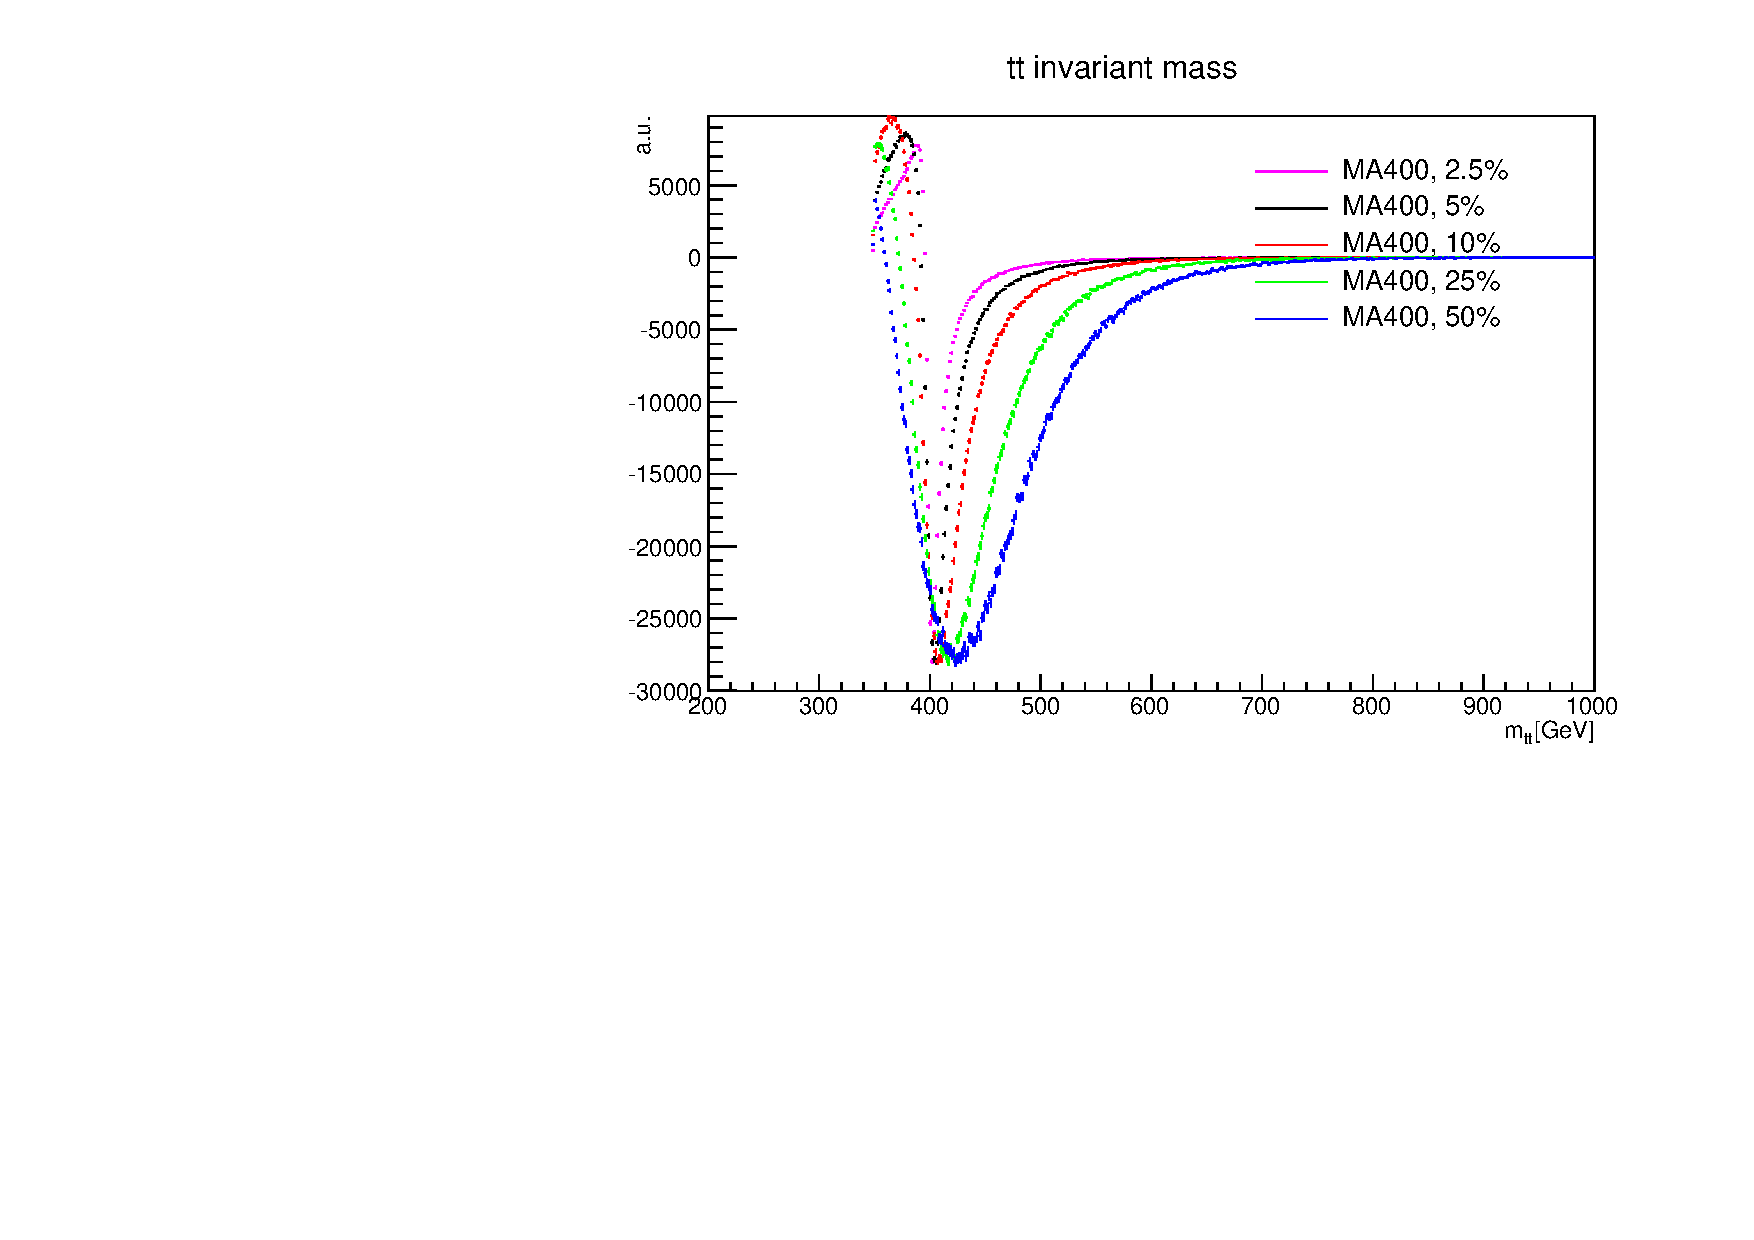
\includegraphics[width=0.4\textwidth]{fig/chapt4/gen_plots/A_int_ljets_M400.pdf}\\
  \caption{Distribution of the $t\bar t$ invariant mass at parton level for a $\mathcal{CP}$-even (left) and a $\mathcal{CP}$-odd (right) particle of mass 400\,GeV for different width hypotheses. The plots correspond to the resonant BSM contribution (top) and interference (bottom).}
  \label{fig:mtt_gen_400}
\end{figure}

\begin{figure} \centering
  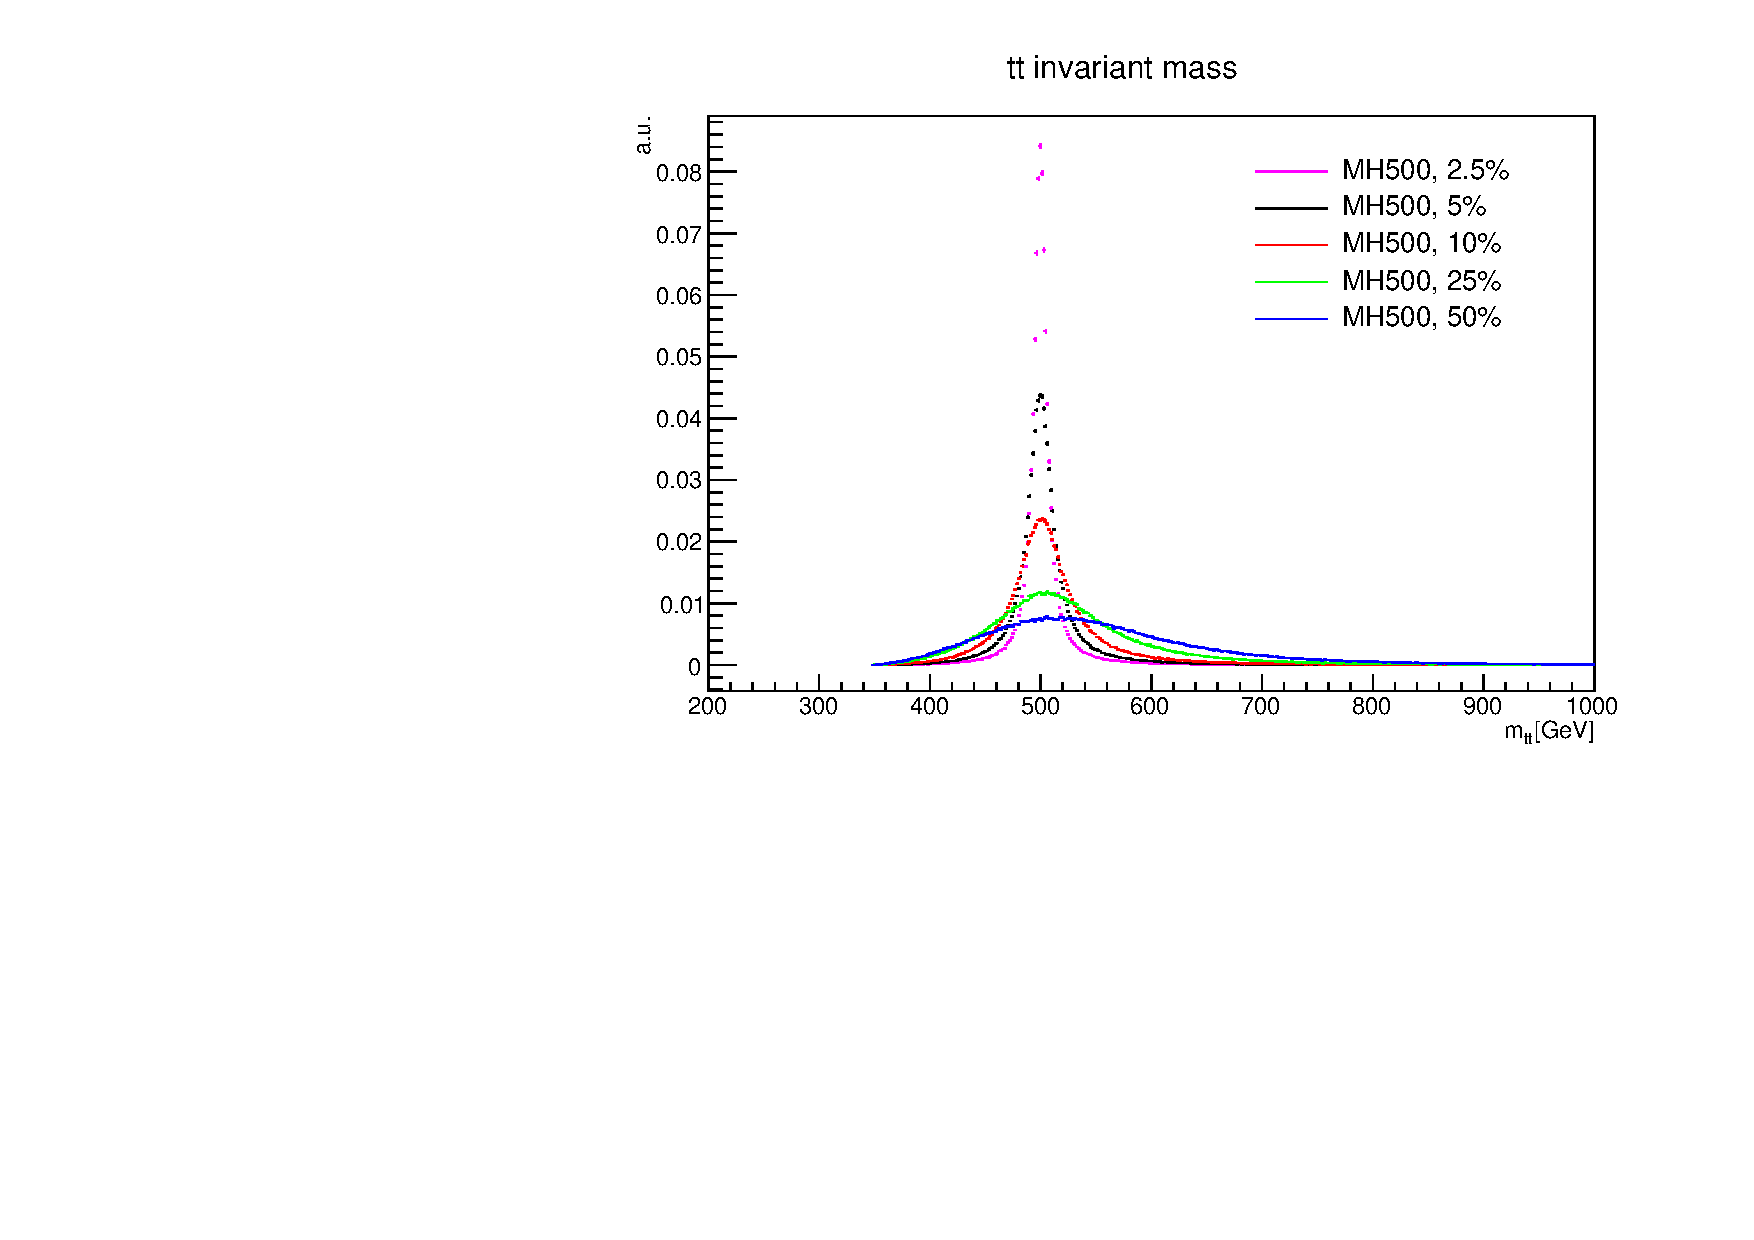
\includegraphics[width=0.4\textwidth]{fig/chapt4/gen_plots/H_res_ljets_M500.pdf}
  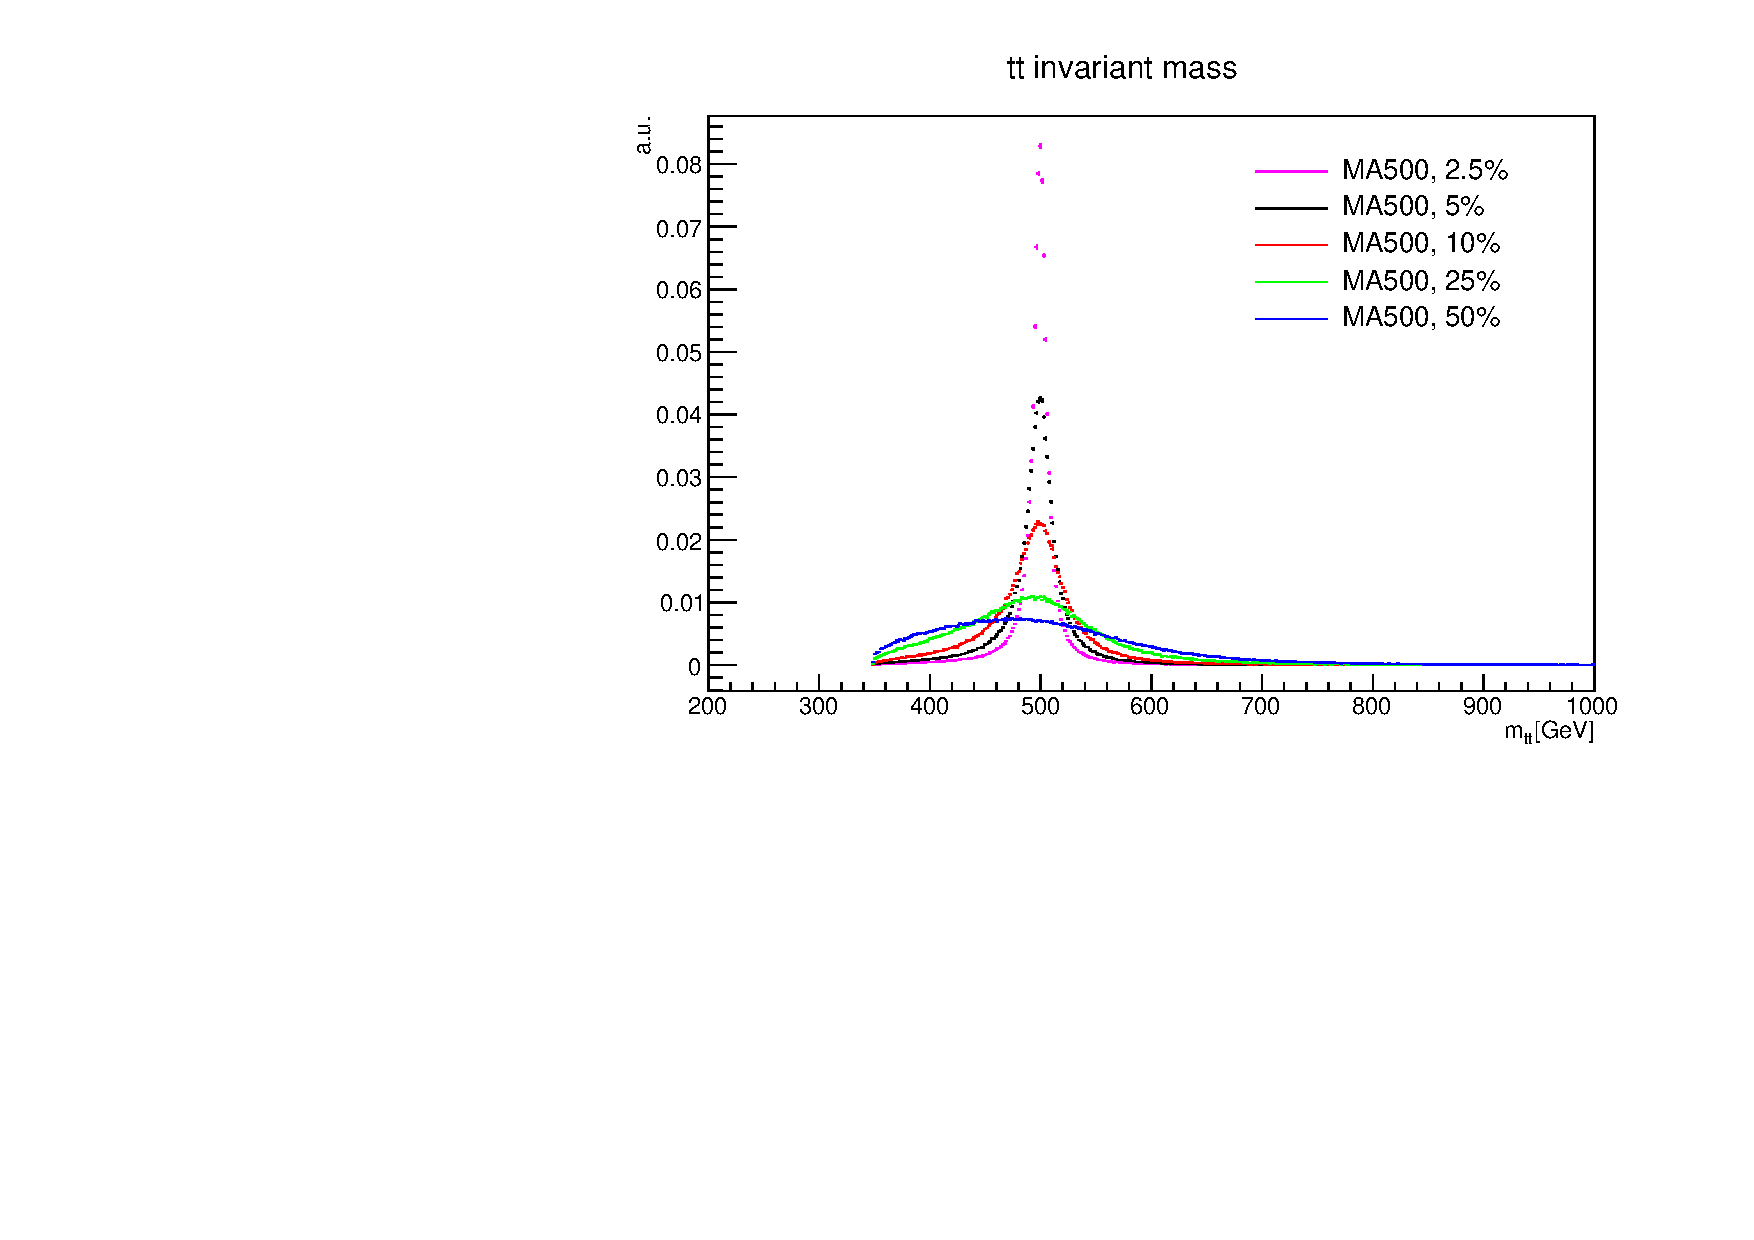
\includegraphics[width=0.4\textwidth]{fig/chapt4/gen_plots/A_res_ljets_M500.pdf}\\
  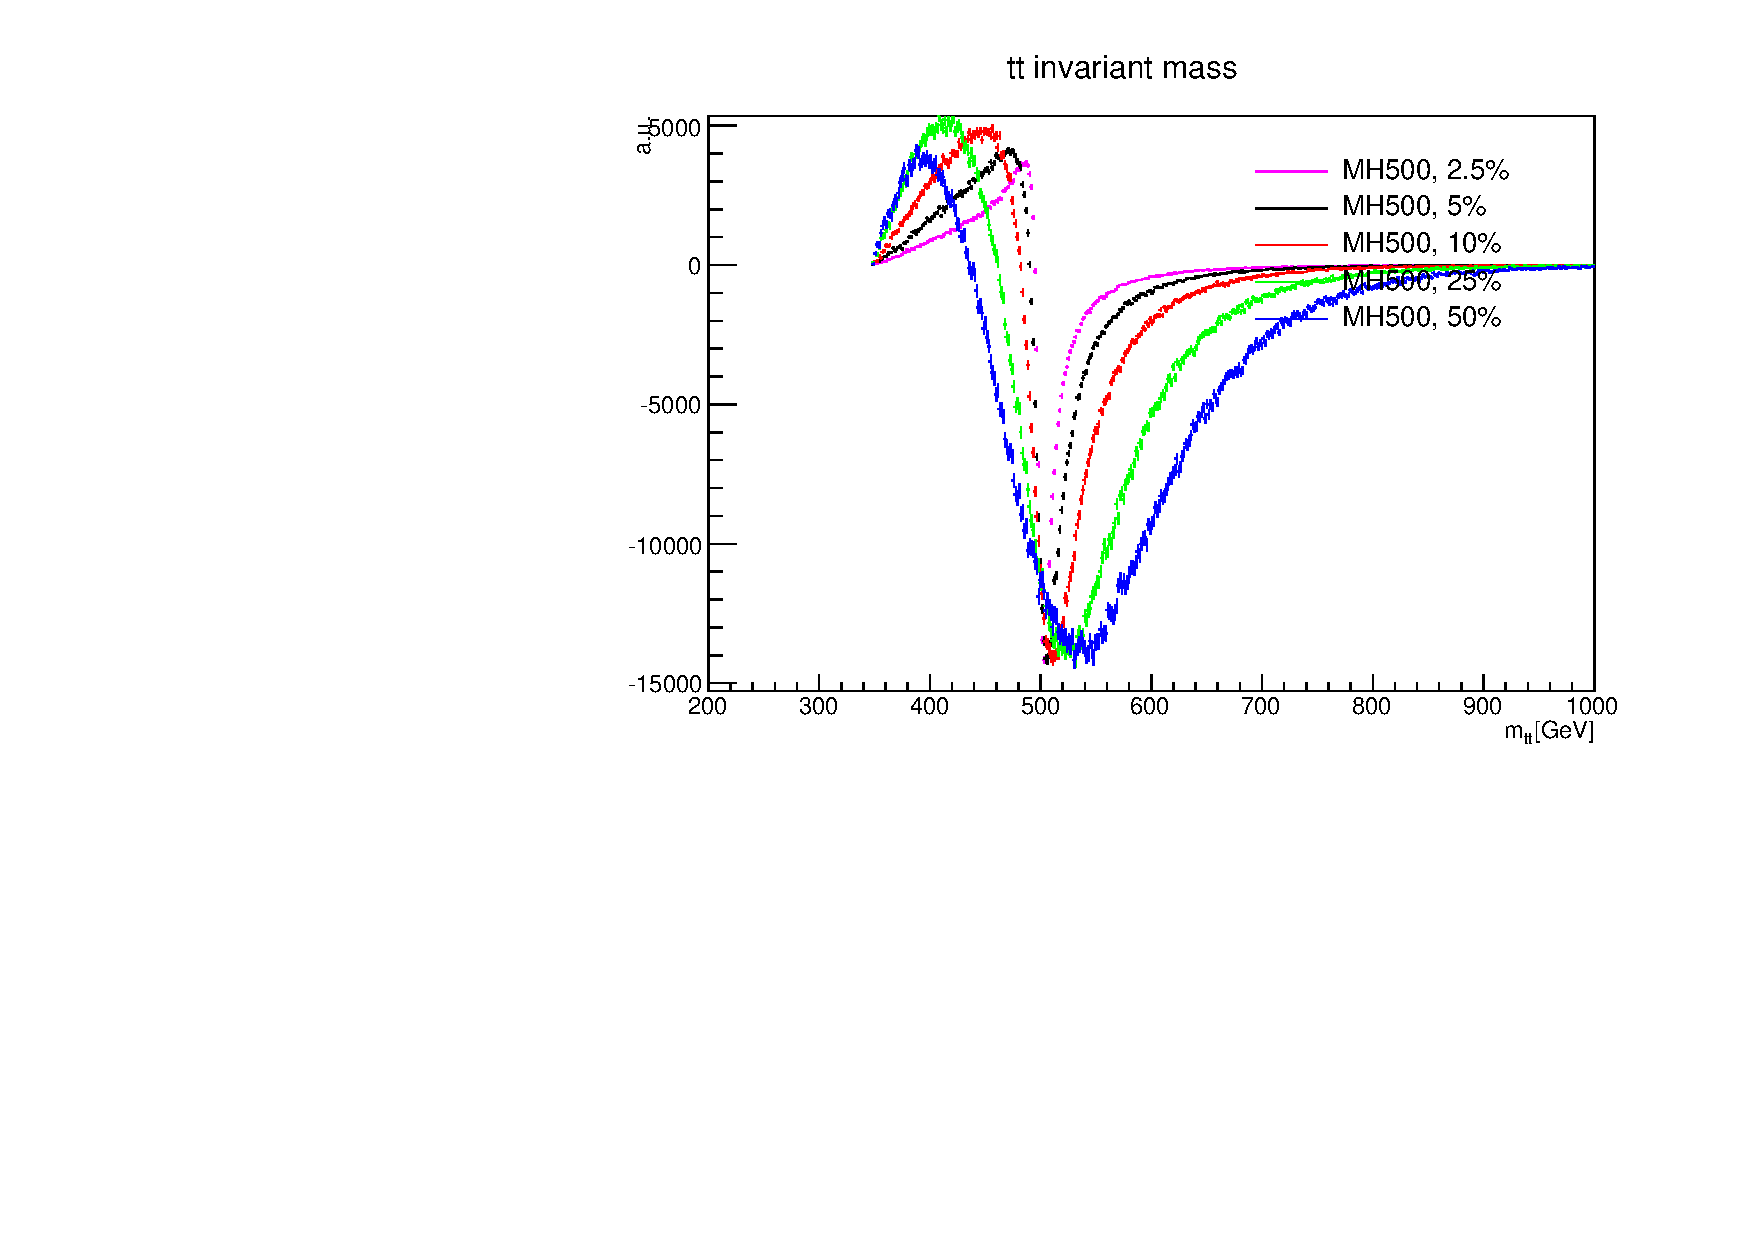
\includegraphics[width=0.4\textwidth]{fig/chapt4/gen_plots/H_int_ljets_M500.pdf}
  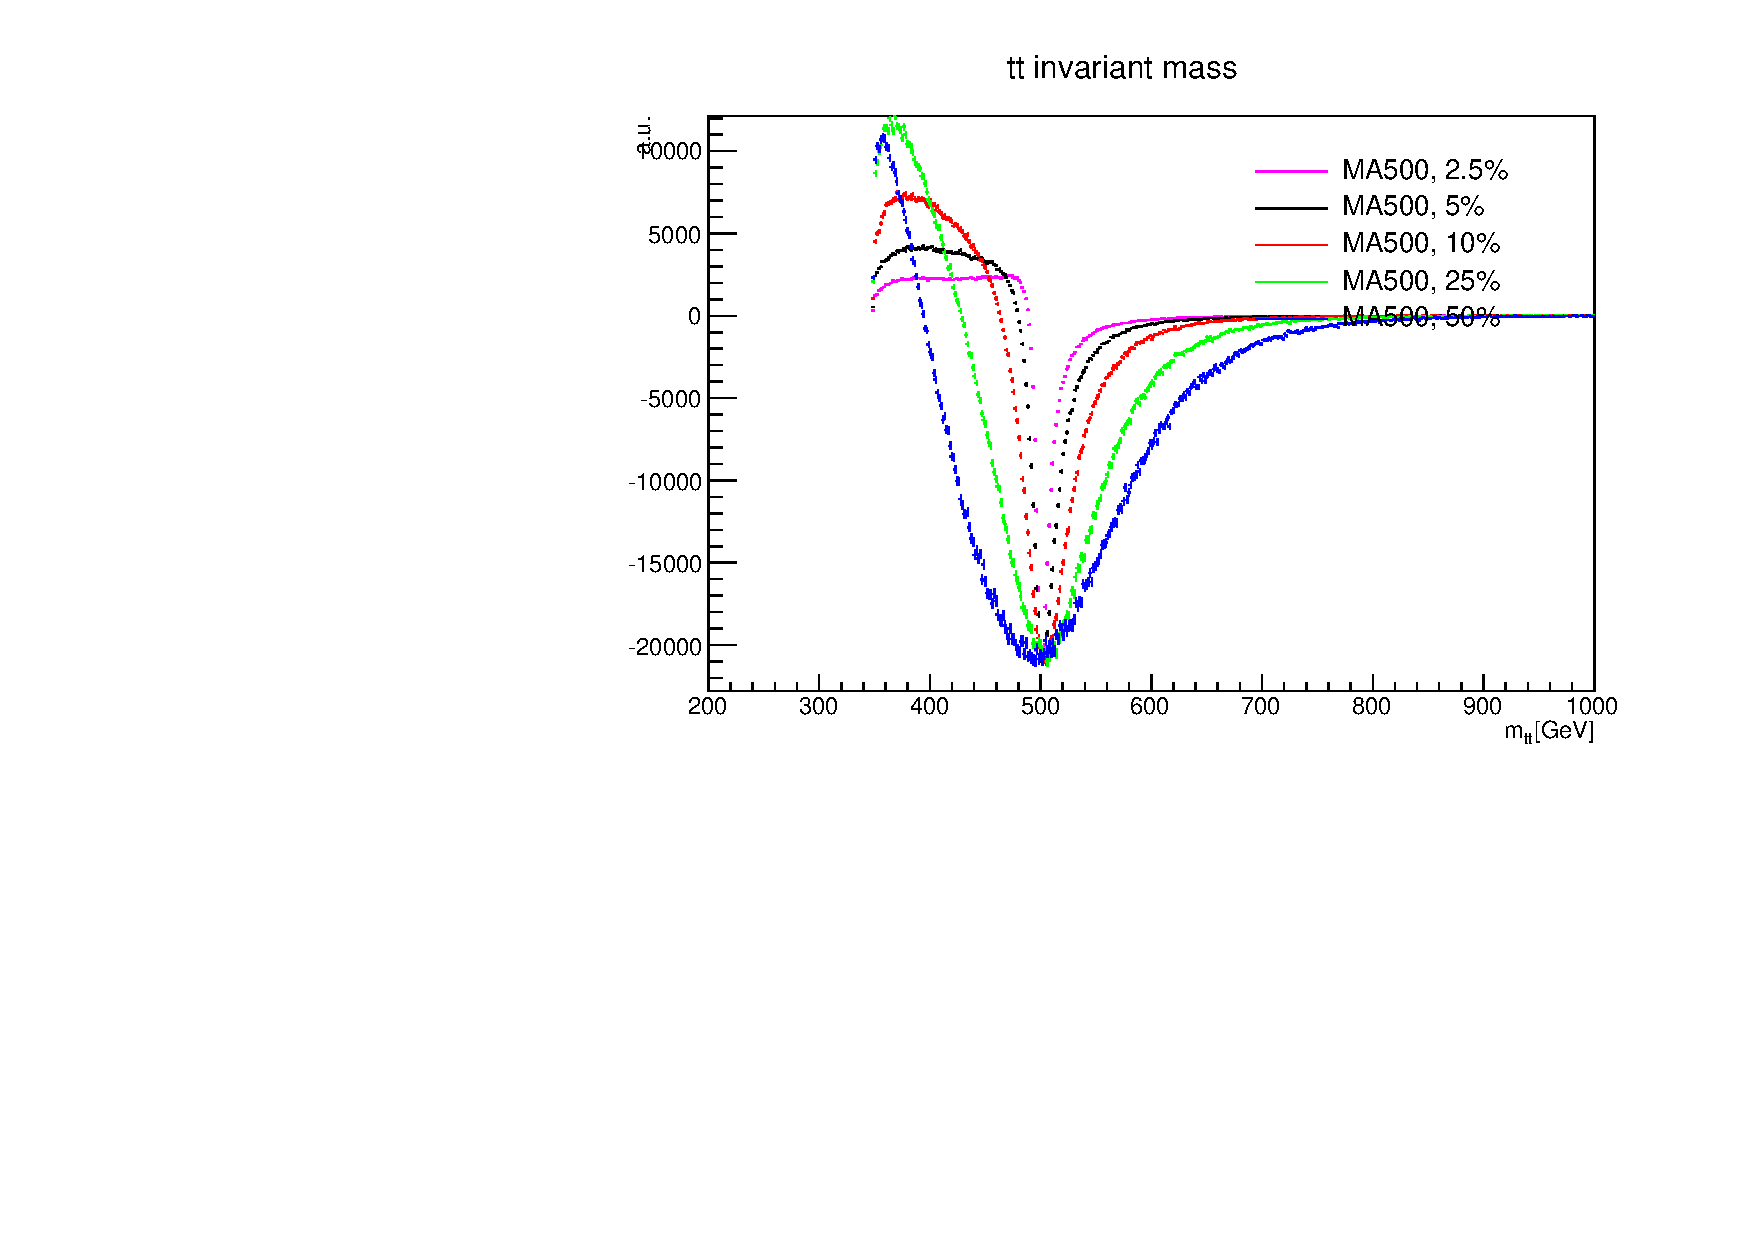
\includegraphics[width=0.4\textwidth]{fig/chapt4/gen_plots/A_int_ljets_M500.pdf}\\
  \caption{Distribution of the $t\bar t$ invariant mass at parton level for a $\mathcal{CP}$-even (left) and a $\mathcal{CP}$-odd (right) particle of mass 500\,GeV for different width hypotheses. The plots correspond to the resonant BSM contribution (top) and interference (bottom).}
  \label{fig:mtt_gen_500}
\end{figure}

\begin{figure} \centering
  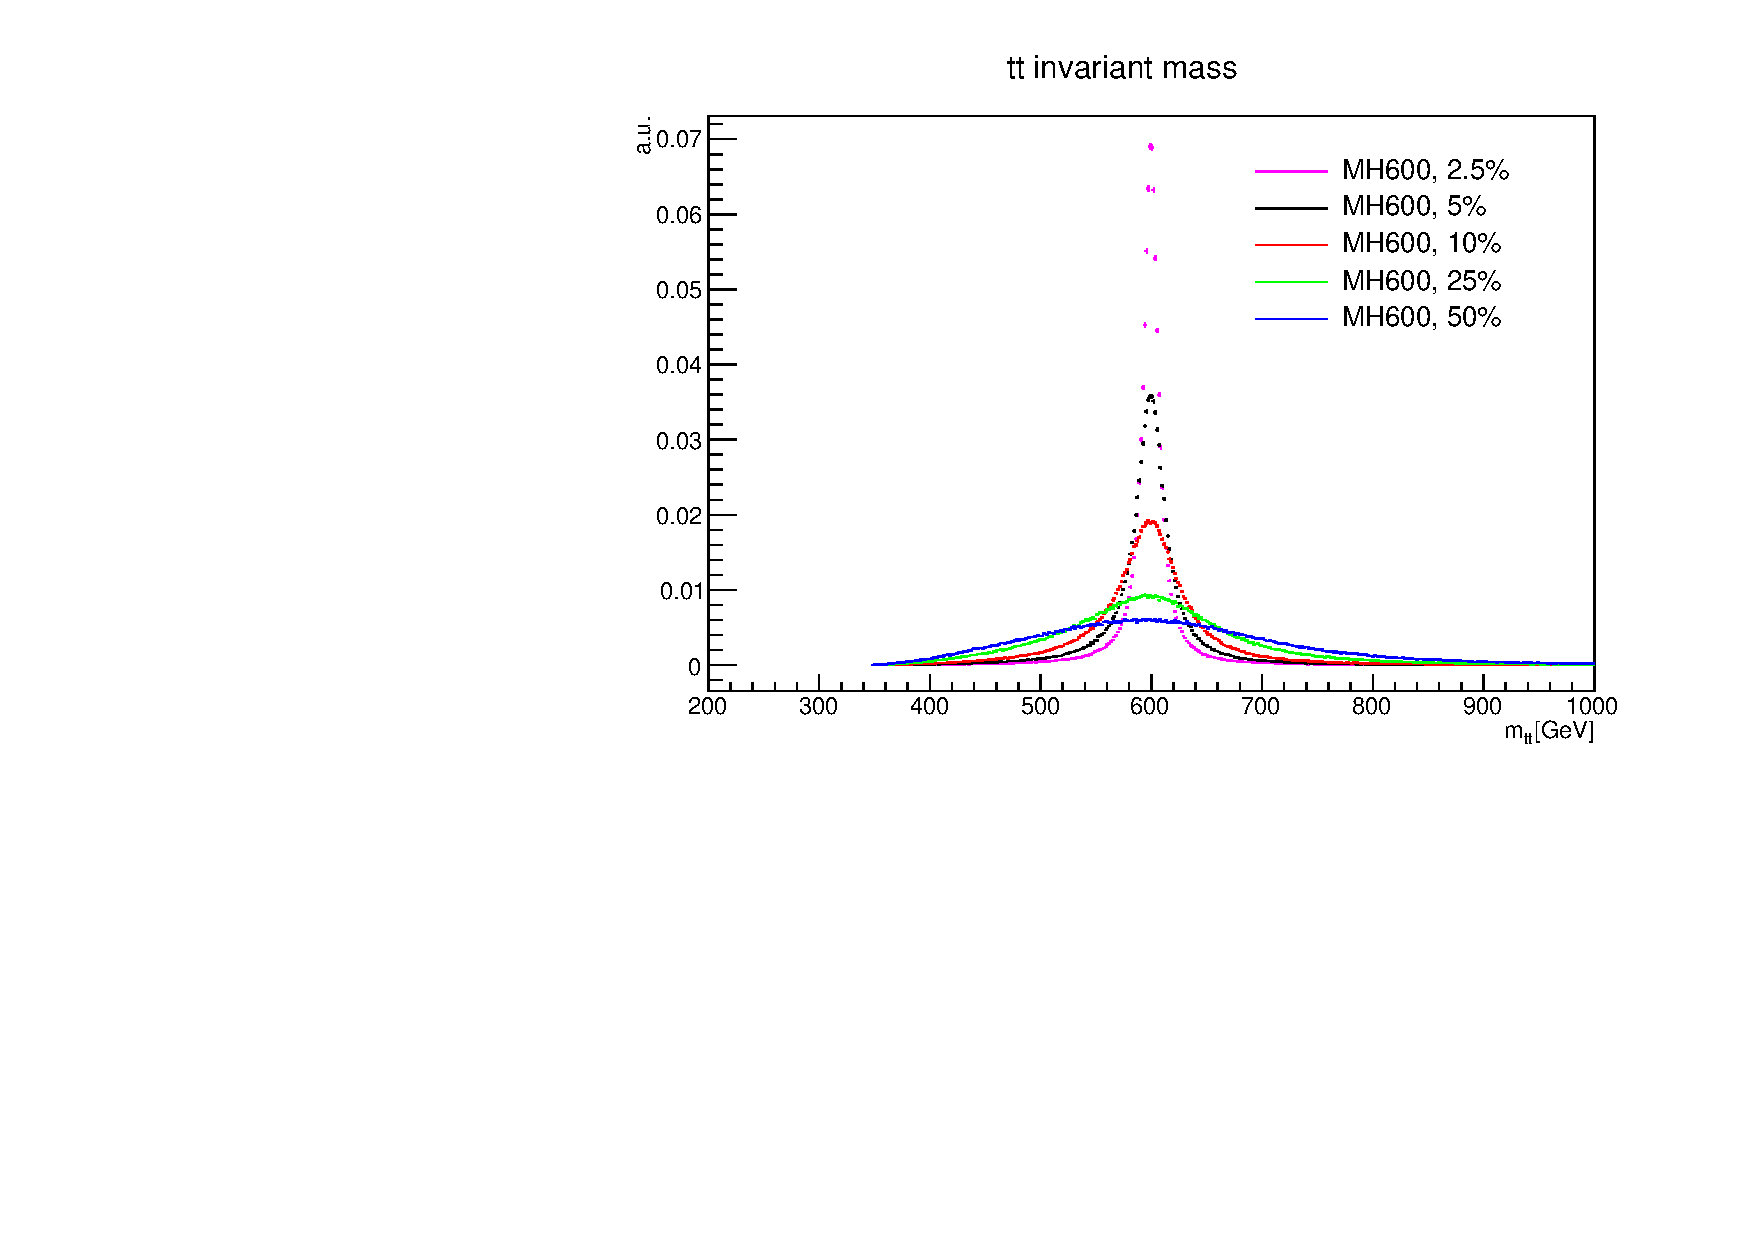
\includegraphics[width=0.4\textwidth]{fig/chapt4/gen_plots/H_res_ljets_M600.pdf}
  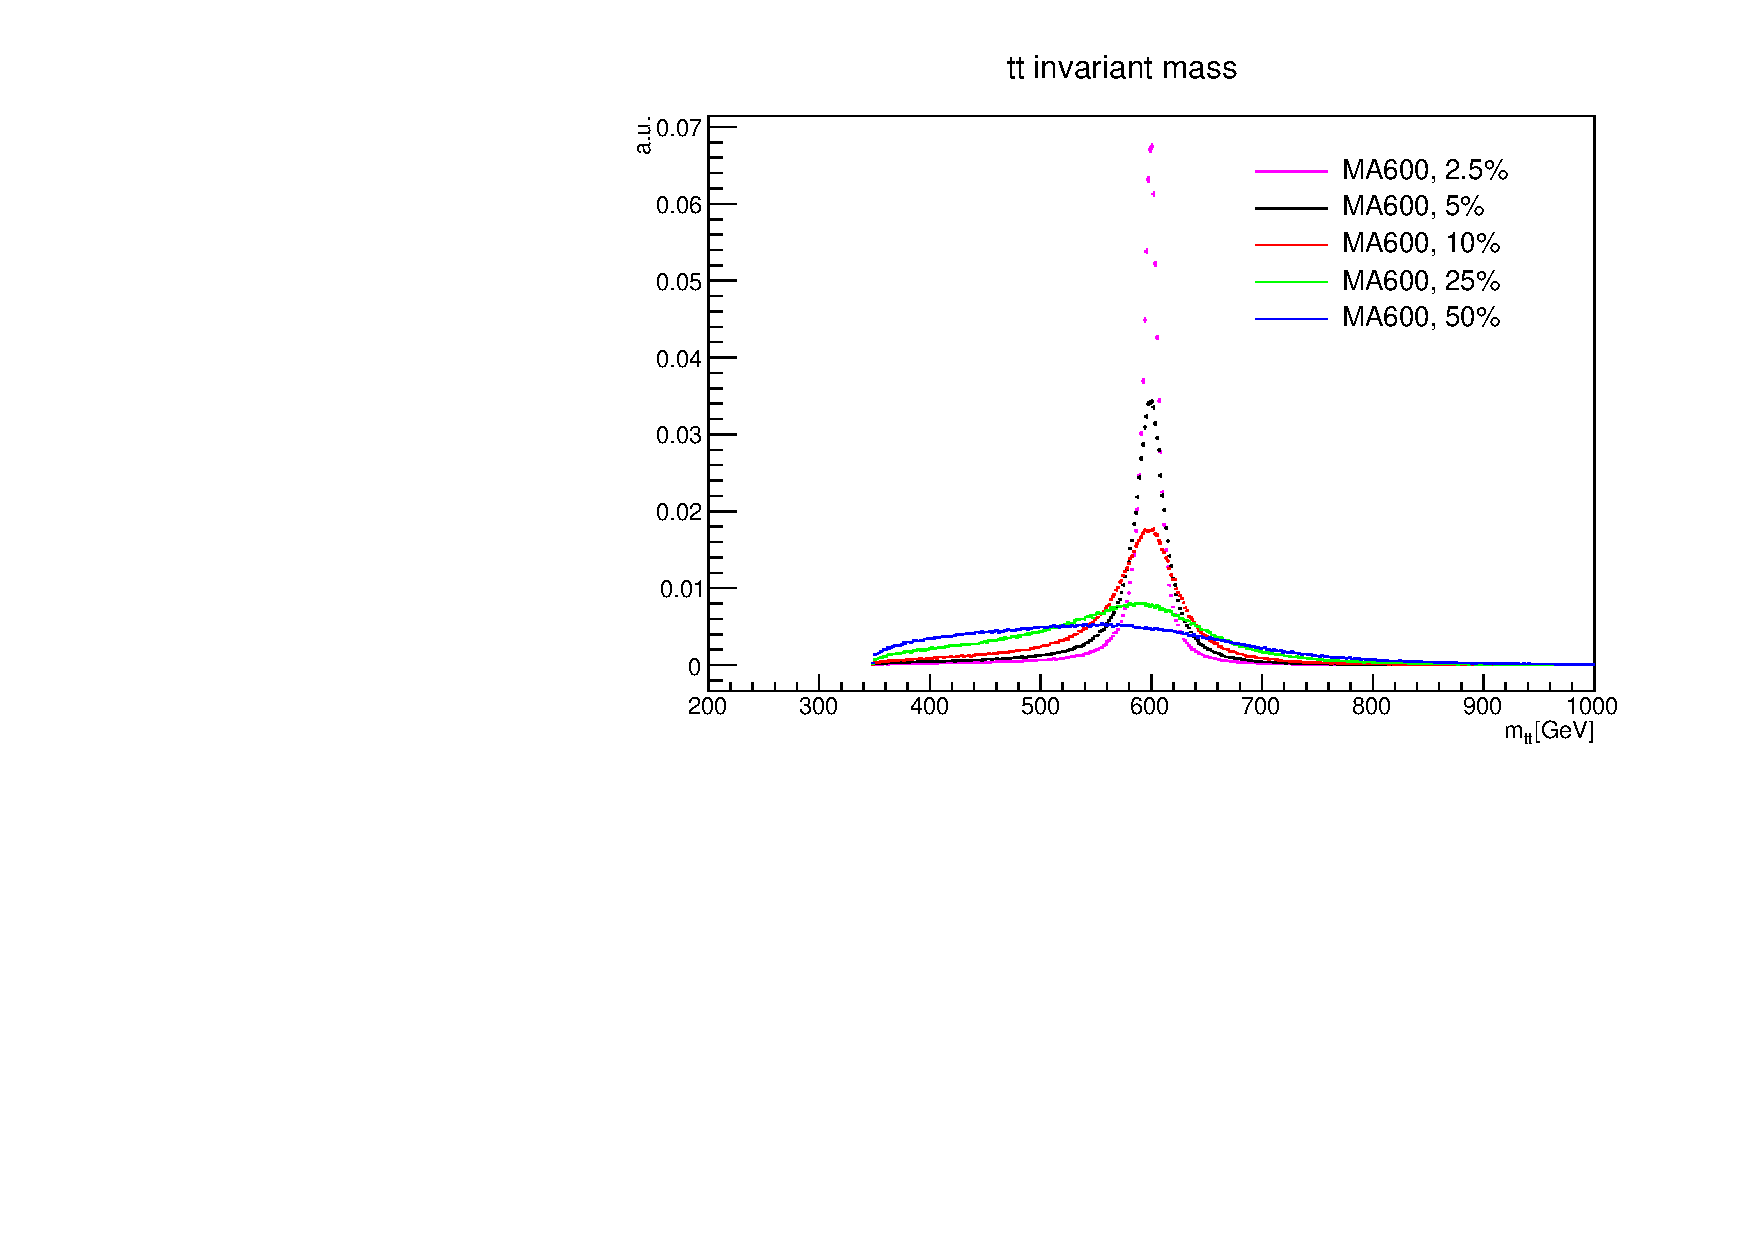
\includegraphics[width=0.4\textwidth]{fig/chapt4/gen_plots/A_res_ljets_M600.pdf}\\
  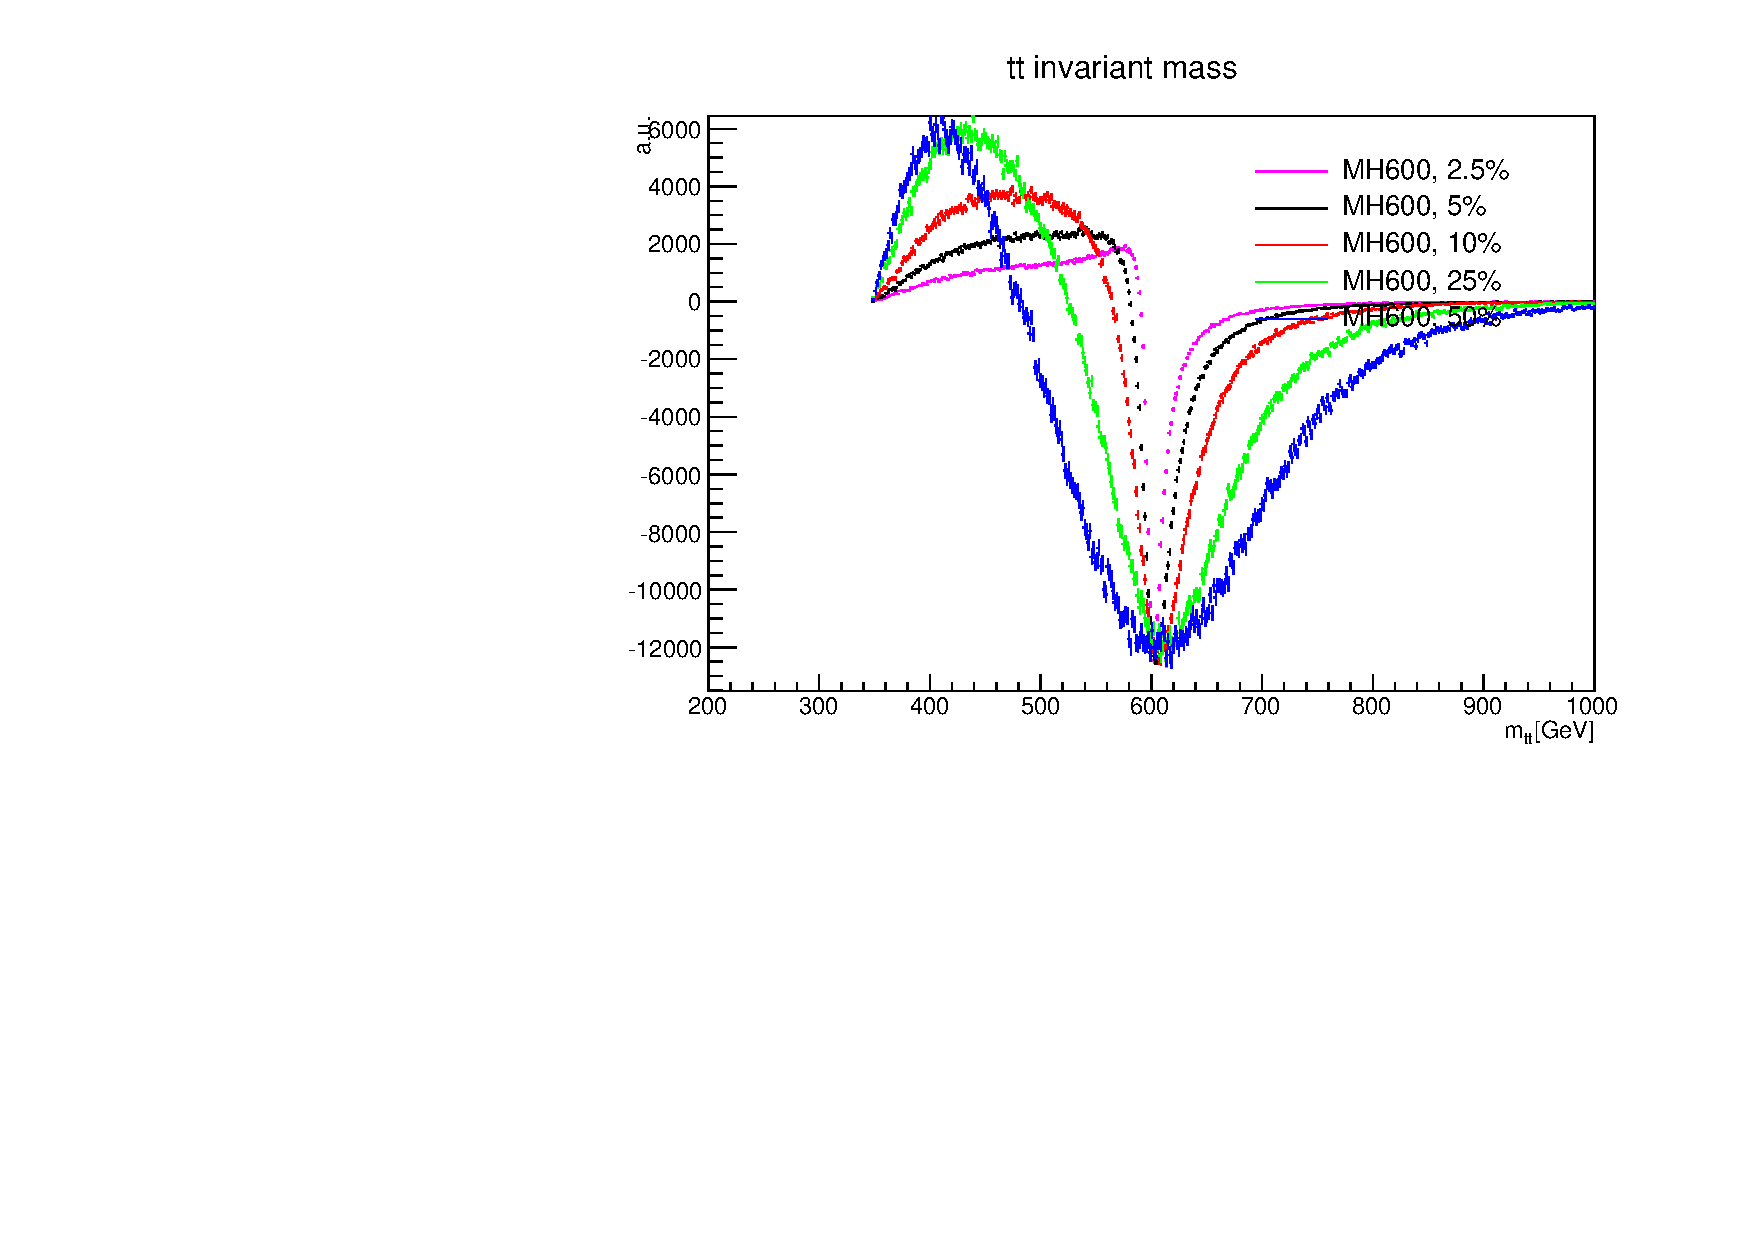
\includegraphics[width=0.4\textwidth]{fig/chapt4/gen_plots/H_int_ljets_M600.pdf}
  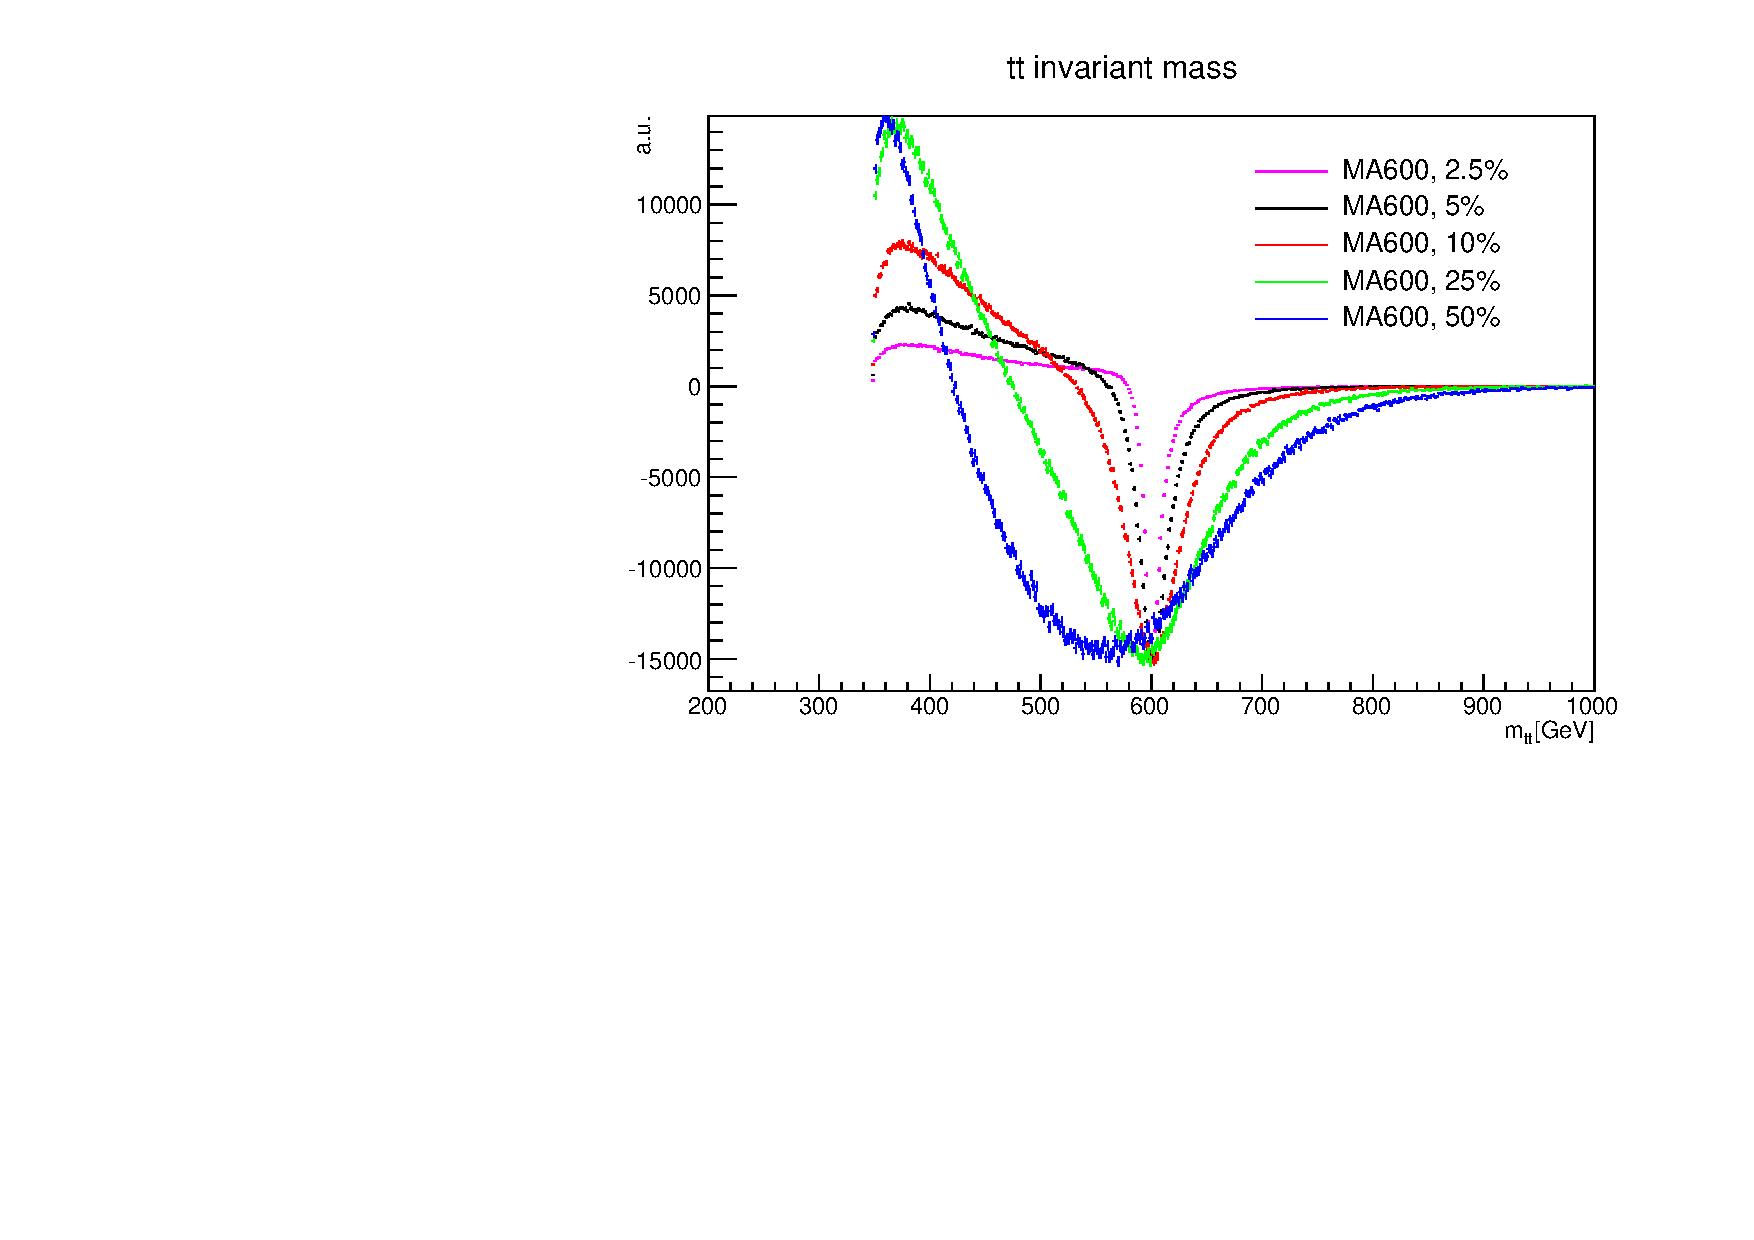
\includegraphics[width=0.4\textwidth]{fig/chapt4/gen_plots/A_int_ljets_M600.pdf}\\
  \caption{Distribution of the $t\bar t$ invariant mass at parton level for a $\mathcal{CP}$-even (left) and a $\mathcal{CP}$-odd (right) particle of mass 600\,GeV for different width hypotheses. The plots are shown for the resonant BSM contribution (top) and interference (bottom).}
  \label{fig:mtt_gen_600}
\end{figure}

\begin{figure} \centering
  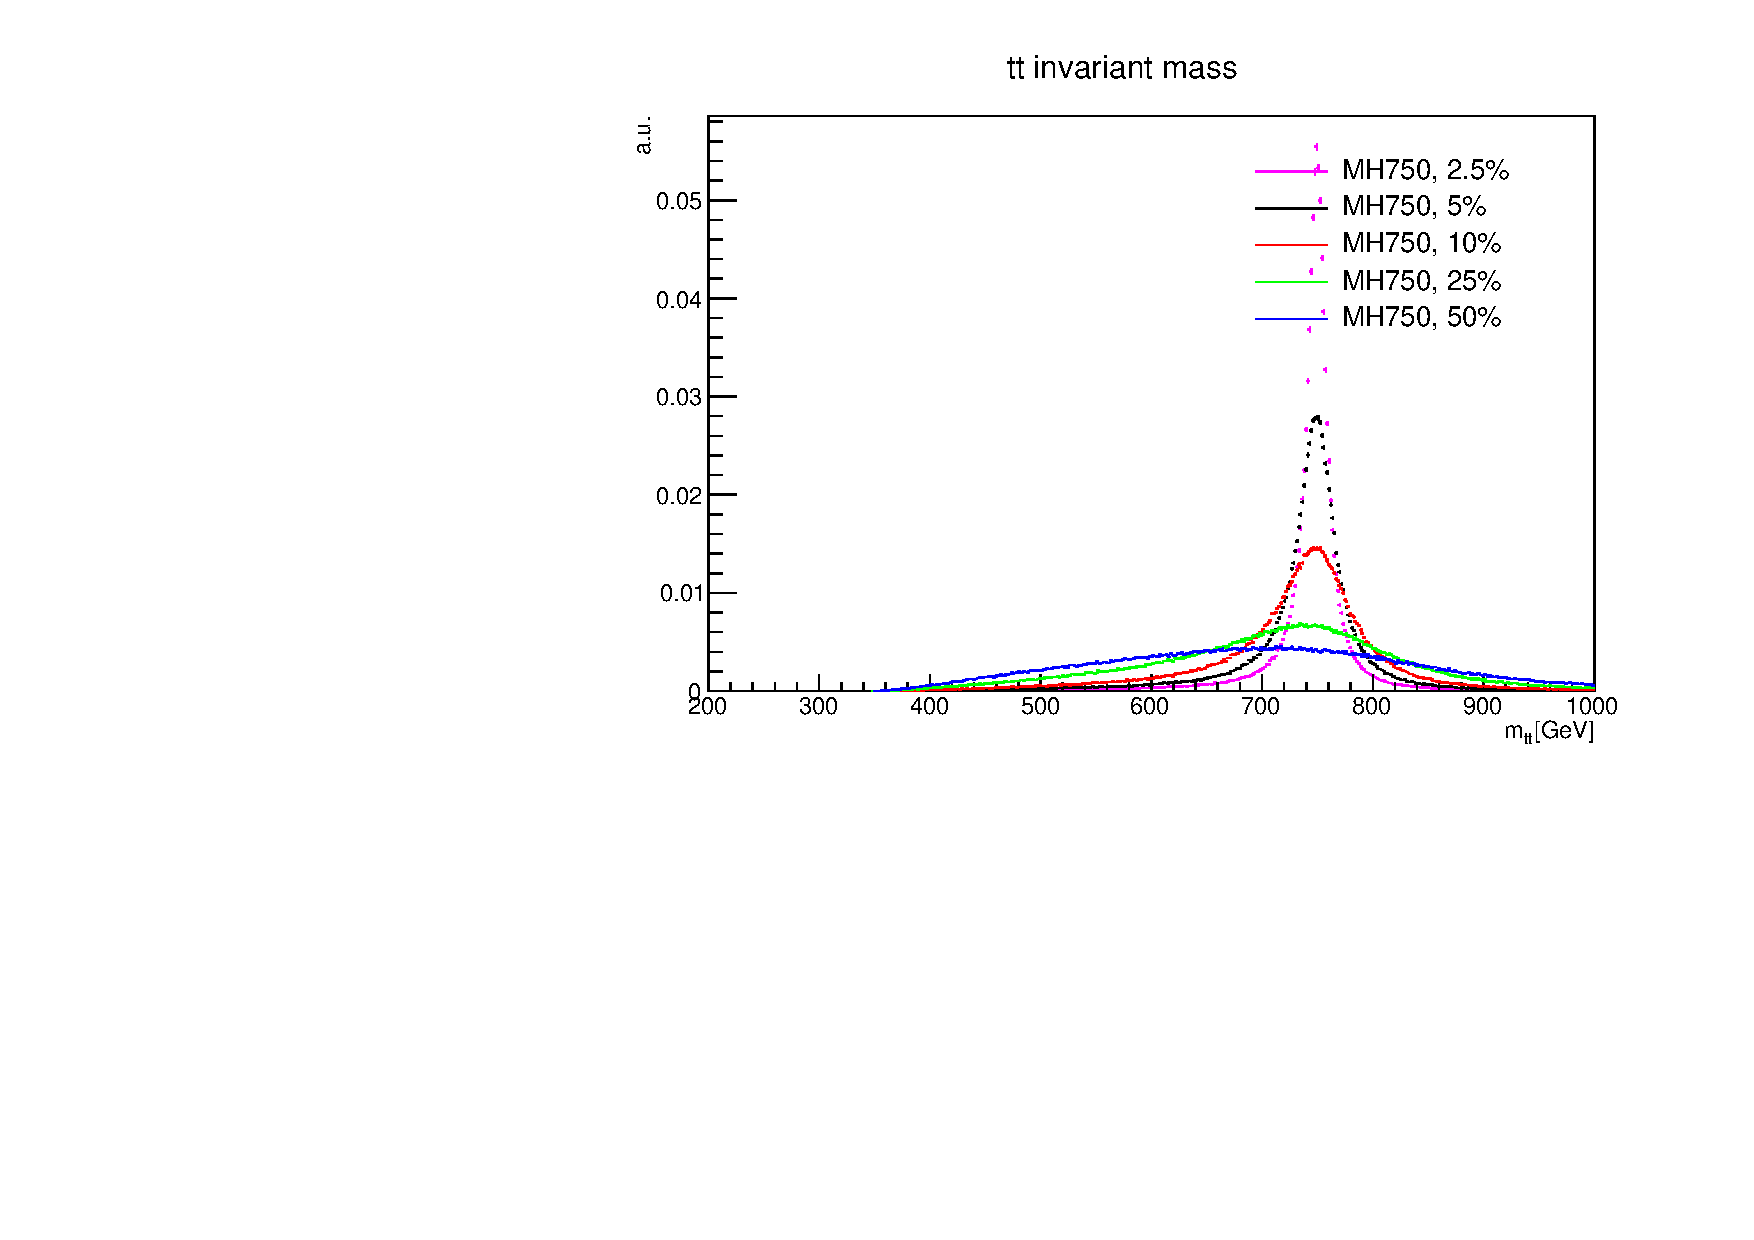
\includegraphics[width=0.4\textwidth]{fig/chapt4/gen_plots/H_res_ljets_M750.pdf}
  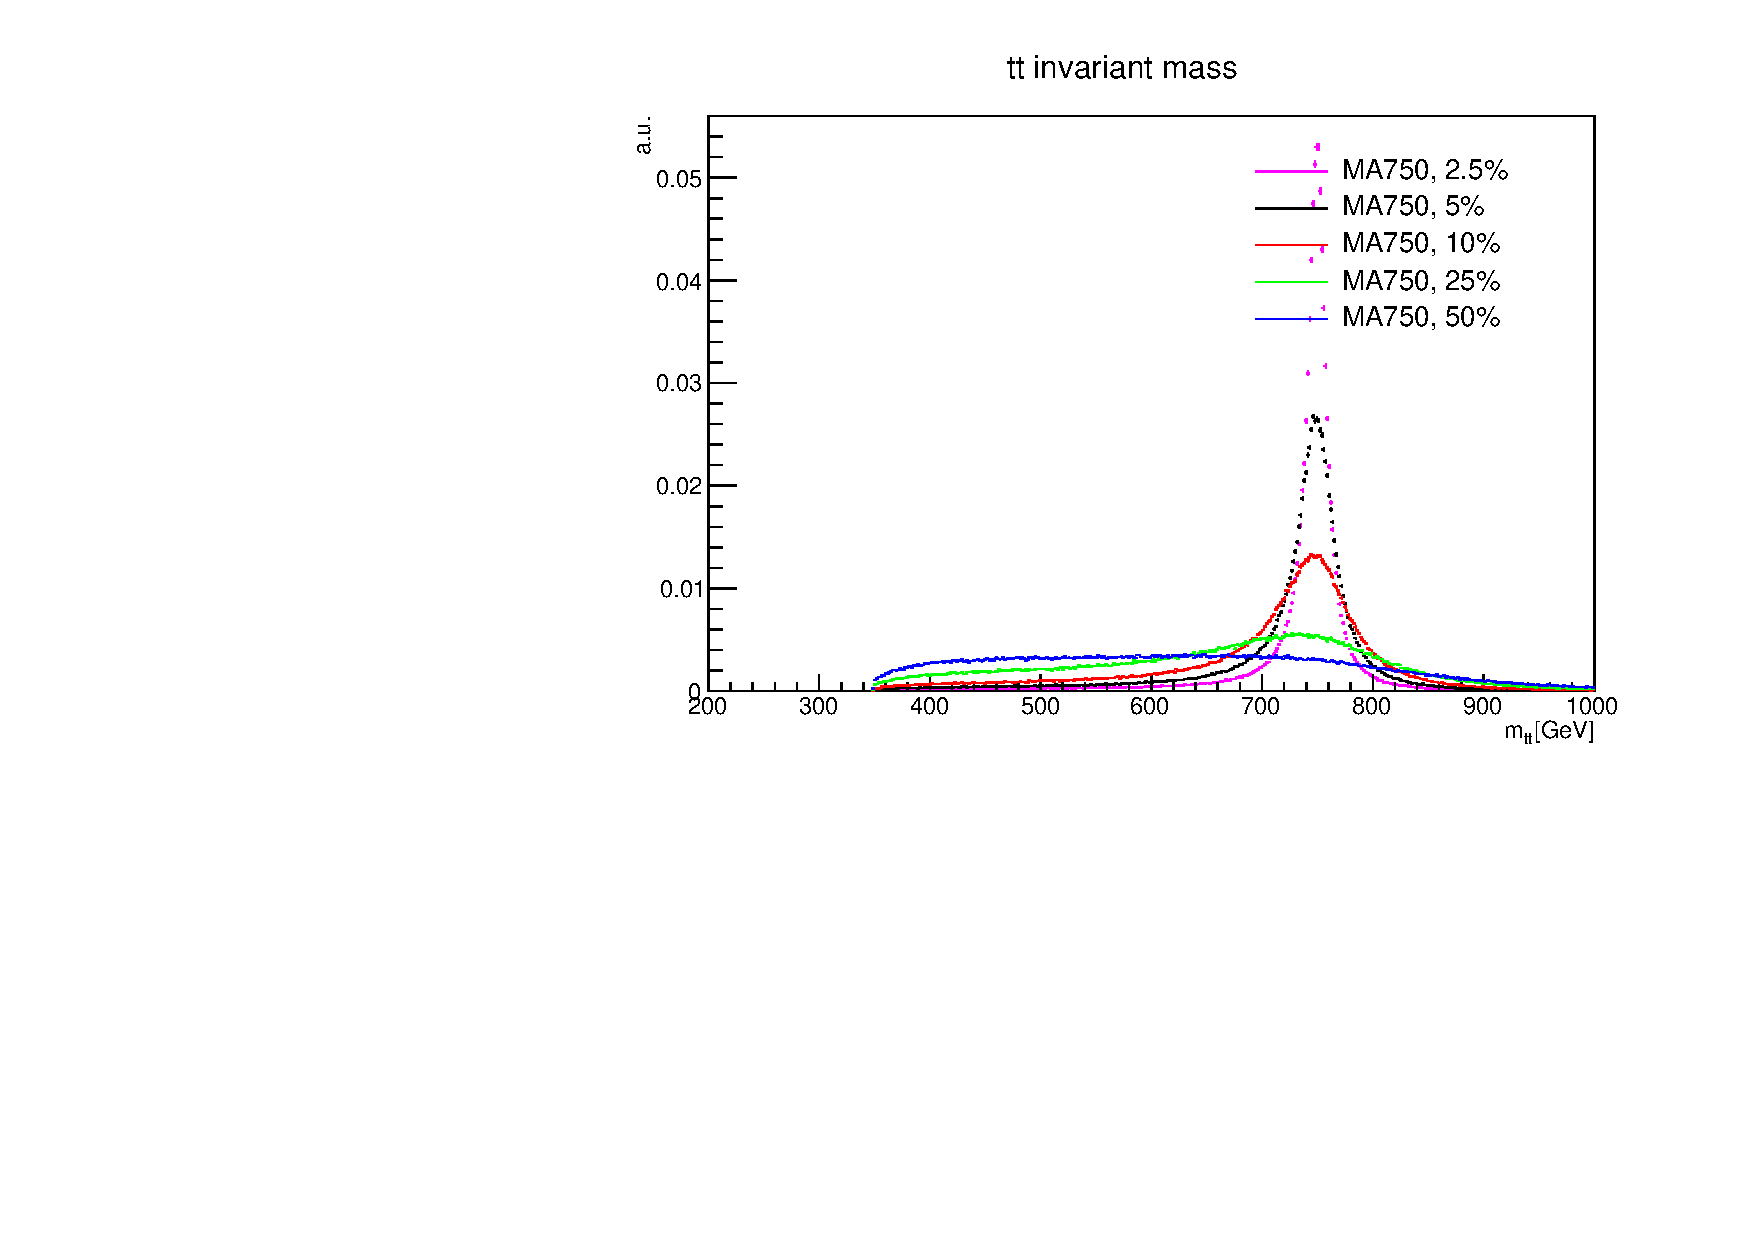
\includegraphics[width=0.4\textwidth]{fig/chapt4/gen_plots/A_res_ljets_M750.pdf}\\
  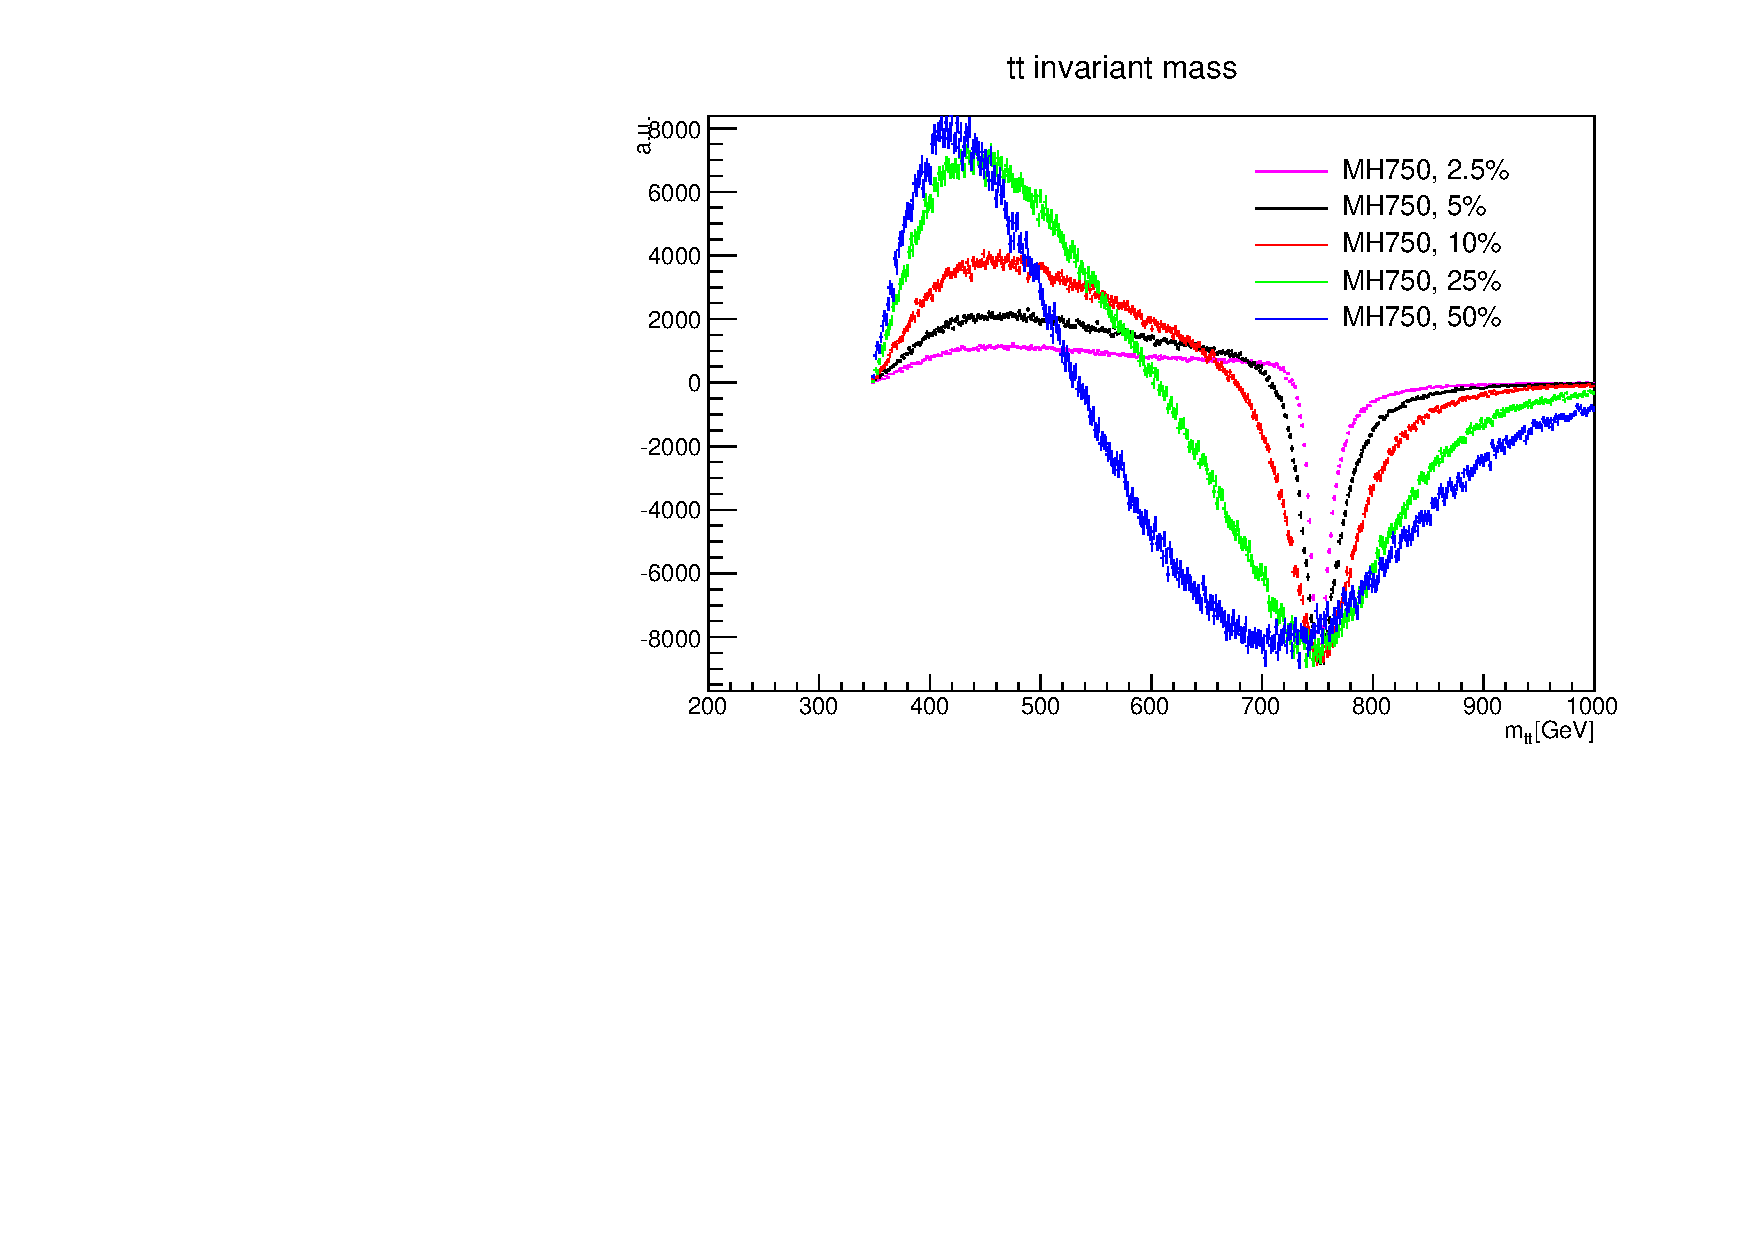
\includegraphics[width=0.4\textwidth]{fig/chapt4/gen_plots/H_int_ljets_M750.pdf}
  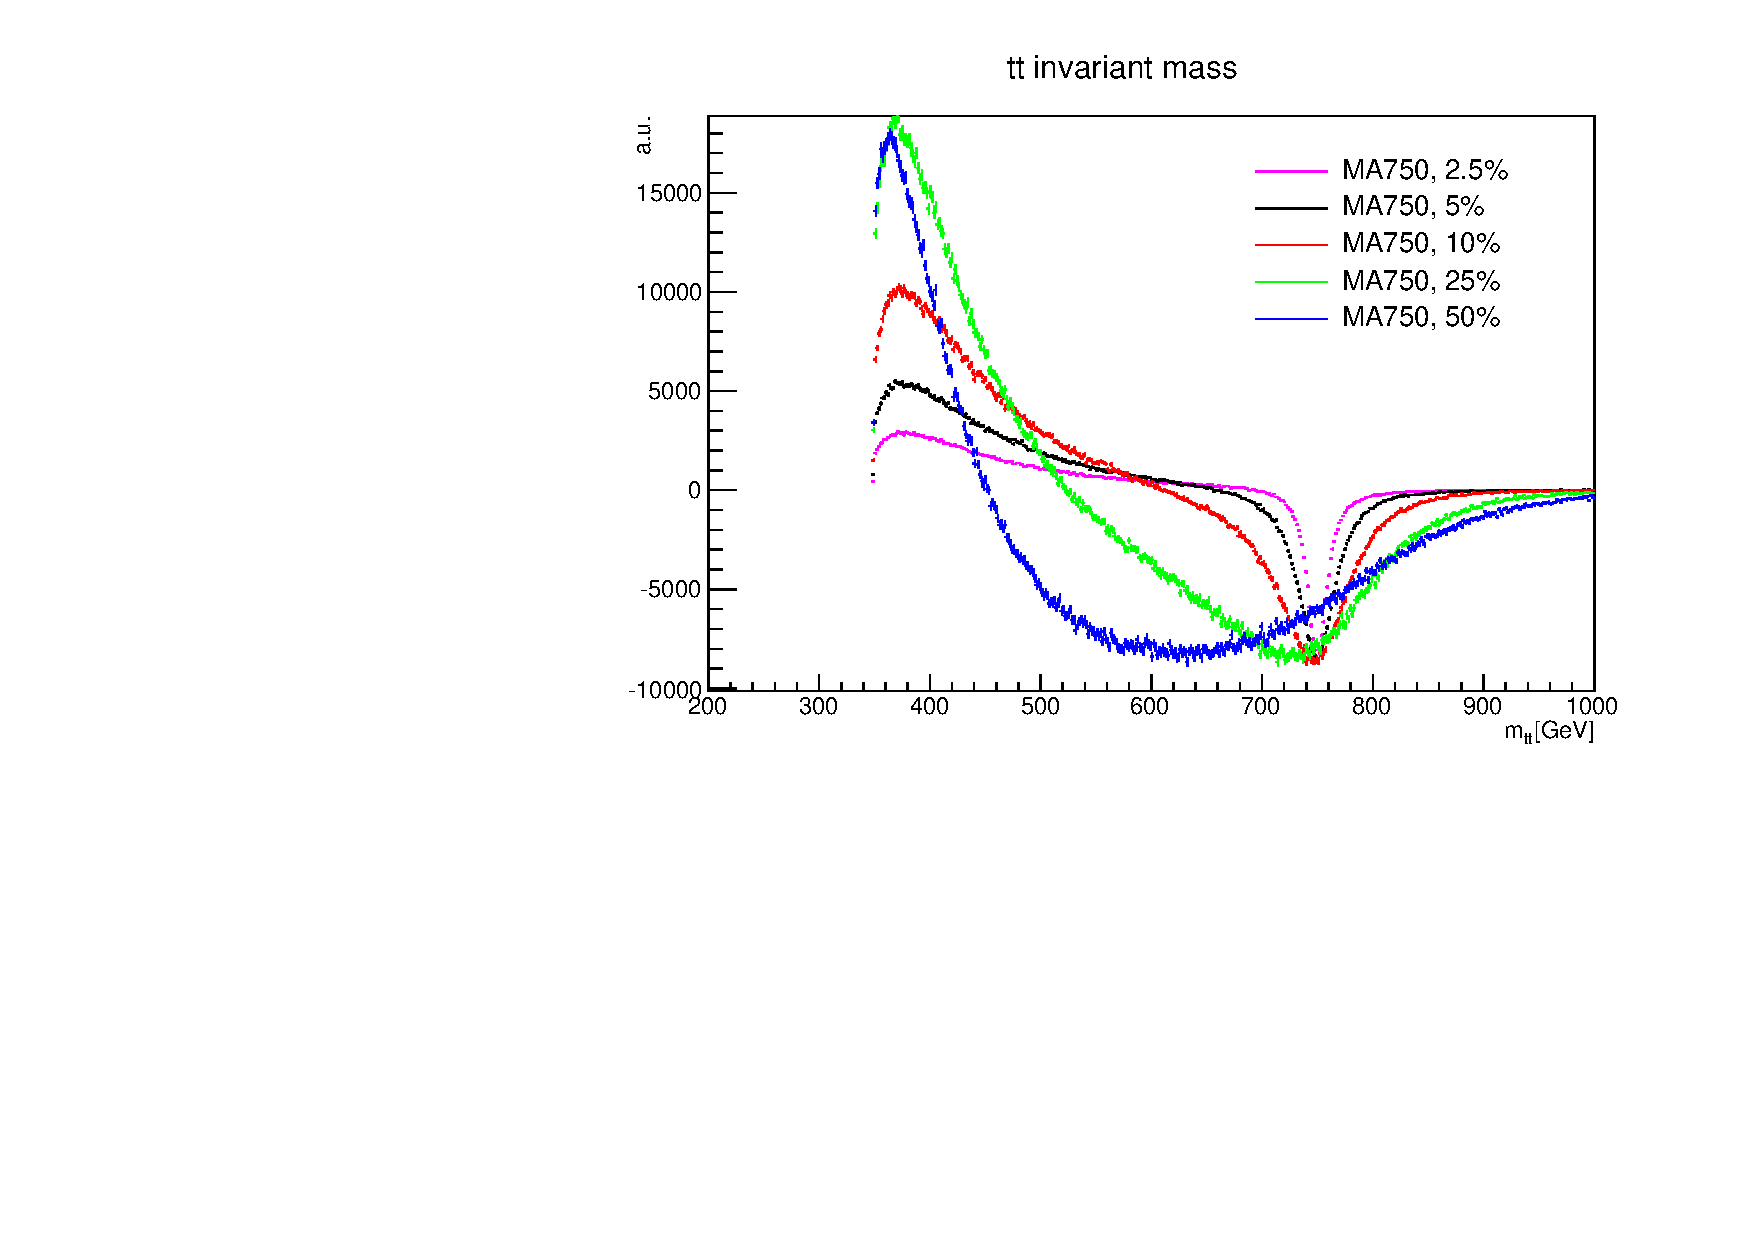
\includegraphics[width=0.4\textwidth]{fig/chapt4/gen_plots/A_int_ljets_M750.pdf}\\
  \caption{Distribution of the $t\bar t$ invariant mass at parton level for a $\mathcal{CP}$-even (left) and a $\mathcal{CP}$-odd (right) particle of mass 750\,GeV for different width hypotheses. The plots are shown for the resonant BSM contribution (top) and interference (bottom).}
  \label{fig:mtt_gen_750}
\end{figure}

%--------------------------------------
\section{Cross section and BR calculation}
To scale the signal leading-order cross section to next-to-next leading order, a number of different types of cross section calculators have been used, as defined in the following section.
\subsection{\textsc{2Hdmc} and \textsc{SusHi}}\label{subsec:sushi}
\textbf{\textsc{2Hdmc:}} Two-Higgs-Doublet Model Calculator~\cite{2hdmc} is a general-purpose calculator based on C++ code, which can be used to study the phenomenology of a general ($\mathcal{CP}$-conserving) two-Higgs doublet model (2HDM), as described in Sec.~\ref{sec:bsm}. \textsc{2Hdmc} provided a user-friendly interface to implement its favourite parameters’ space for the Higgs potential. A user has full control over the Yukawa sector through changing the coupling. The Higgs masses, type of the model (type I and type II), alignment limit condition $\sin (\alpha-\beta)$, the ratio of the vacuum expectation values of the doublet in 2HDM ($\tan\beta$), the scalar mass matrix, m$^{2}_{12}$, etc. can be specified with full freedom. The output of the \textsc{2Hdmc} consists of a check on the theoretical properties of the model, such as $\mathcal{CP}$-conservation, positivity and stability of the potential, and the tree level unitarity and perturbativity. \textsc{2Hdmc} can be used to calculate the Higgs decay widths and branching ratios.

This work uses \textsc{2Hdmc} to calculate decay widths of the neutral Higgs sector, scalar (H), or pseudo-scalar (A), by making an iteration over the $\tan\beta$ values. The signal samples have been generated for heavy Higgs (scalar and pseudo-scalar) using \textsc{MadGraph} for fixed masses and widths. The considered masses are 400, 500, 600, and 750\,GeV; for each mass, five width values (1, 5, 10, 25, 50)\% are taking into account. \textsc{2Hdmc} uses fixed values for charged Higgs mass (mC = 600\,GeV), scalar or pseudo-scalar Higgs mass (mA/H = 400\,GeV), and sin ($\alpha - \beta$) = 1, $\lambda_{6,7}$ = 0 and $m^{2}_{12} = m^{2}_{A}\tan\beta/(1 + \tan^{2}\beta)$. An iteration of the $\tan\beta$ values is conducted and the one that provides the corresponding width considered for signal generation in \textsc{MadGraph} is selected. The same procedure is repeated for all masses. The selected $\tan\beta$ values are further used in the \textsc{SusHi} as input.
   
%-------------------------------------
\textbf{\textsc{SusHi:}} Supersymmetric Higgs~\cite{sushi} is a Fortran-based program, designed to calculate inclusive Higgs boson production cross sections up to NNLO QCD through gluon fusion and bottom-quark annihilation in the Standard Model (SM), general Two-Higgs-Doublet Models (2HDM), the Minimal Supersymmetric Standard Model (MSSM), and its next-to-minimal extension (NMSSM). The program can also be used to calculate differential cross sections with respect to the Higgs transverse momentum $p_{T}$ and (pseudo-)rapidity y($\eta$). \textsc{SusHi} can be linked with the \textsc{2Hdmc} calculator for performing 2HDM calculation, with FeynHiggs for the MSSM Higgs masses calculations, and many more. In this work, \textsc{SusHi} links with \textsc{2Hdmc} for neutral Higgs LO and NNLO cross section calculations in 2HDM/hMSSM and incorporates the PDF effects by using external PDF sets (\textsc{Nnpdf30}). Factorization and normalization scales are fixed with respect to the neutral Higgs mass ($\mu_{F/R} = m_{A/H}/2$). The output card of the \textsc{2Hdmc} is used as the input in \textsc{SusHi} with 2HDM model in the physical Higgs basis. The $\tan\beta$ value that corresponds to a certain width is used as a coupling modifier ($g_{A/H}\rightarrow t\bar{t}$) in the \textsc{MadGraph} parameter card. The output of LO cross sections from \textsc{SusHi} is comparable with the \textsc{MadGraph} cross sections shown in table~\ref{table:mg_sushi_compare}. The k-factor is calculated as a ratio of NNLO \textsc{SusHi} cross sections to LO. The results are interpreted to weight the SM cross sections with these k-factors. NNLO \textsc{SusHi} cross sections to LO \textsc{MadGraph} with errors is plotted in Fig.~\ref{fig:k_factor}.
\begin{landscape}
\begin{table}[ht]
\caption{Comparison of leading order cross section from \textsc{MadGraph} and \textsc{SusHi} for pseudo-scalar resonance with masses 400, 500, and 600\,GeV and scalar mass = 700\,GeV. The typical k-factor shows universality for a single mass point that is calculated as the ratio of NNLO from \textsc{SusHi} and \textsc{MadGraph} LO cross sections.}
\centering
\begin{tabular}{| c | c | c | c | c | c | c | c | c | c |}
\hline\hline
Mass (GeV) & Width (GeV) & $\tan\beta$ & $\frac{1}{\tan\beta}$ & LO $\sigma(MG)$ pb & LO $\sigma(\textsc{SusHi})$ pb & NNLO $\sigma(\textsc{SusHi})$ pb & BR (A$\rightarrow t\bar{t}$) & K = $\frac{NNLO \sigma(\textsc{SusHi})}{\sigma(MG)}$ \\ 
\hline\hline
\multirow {6}{*}{400}& 4.002 & 1.908 &  0.52410901467 & 3.641$\pm$0.003587 &  3.63478$\pm$0.0000 & 7.71736$\pm$0.00795 & 9.880$10^{-01}$ & 2.12$\pm$0.003\\
\cline{2-9}
& 10 & 1.2068 & 0.82863771958 & 9.096$\pm$0.009417 & 9.13195$\pm$0.0 & 19.26195$\pm$0.01987 & 9.950$10^{-01}$ & 2.118$\pm$0.009417\\
\cline{2-9}
& 19.49 & 0.8645 & 1.15673799884 & 17.76$\pm$0.01694 & 17.82577$\pm$0.00001 & 37.51884$\pm$0.03872 & 9.960$10^{-01}$ & 2.113$\pm$0.0030\\
\cline{2-9}
& 38.99 & 0.6113 & 1.63585800752 & 35.47$\pm$0.03629 & 35.68351$\pm$0.00002 & 75.01936$\pm$0.07743 & 9.963$10^{-01}$ & 2.115$\pm$0.0031\\
\cline{2-9}
& 97.52 & 0.3865 & 2.5873221216 & 88.86$\pm$0.07161 & 89.31375$\pm$0.00005 & 187.64029$\pm$0.19371 & 9.963$10^{-01}$ & 2.112$\pm$0.0028\\
\cline{2-9}
& 195 & 0.2733 & 3.65898280278 & 177.3$\pm$0.1163 & 178.65641$\pm$0.00009 & 375.25547$\pm$0.38741 & 9.963$10^{-01}$ & 2.117$\pm$0.0026\\
\hline \hline
\multirow {6}{*}{500} & 5.032 & 2.12 & 0.4716981132 & 0.9349$\pm$0.0007767 & 0.94977$\pm$0.0000 & 1.90812$\pm$0.00263 & 9.627$10^{-01}$ & 2.041$\pm$0.0033\\
\cline{2-9}
&12.4 & 1.3506 & 0.73746312684 & 2.291$\pm$0.002217 & 2.32963$\pm$0.000 & 4.66077$\pm$0.00648 &9.854$10^{-01}$ & 2.034$\pm$0.0034\\
\cline{2-9}
&24.81 & 0.9549 & 1.04723007645 & 4.613$\pm$0.00459 & 4.65371$\pm$0.000 & 9.29670$\pm$0.01297 & 9.918$10^{-01}$ & 2.015$\pm$0.0035\\
\cline{2-9}
&49.61 & 0.6752 & 1.48104265403 & 9.235$\pm$0.009654 & 9.30136$\pm$0.00001 & 18.56738$\pm$0.02594 & 9.947$10^{-01}$ & 2.011$\pm$0.0035\\
\cline{2-9}
&124.0 & 0.4271 & 2.34137204402 & 23.08$\pm$0.02179 & 23.23658$\pm$0.00001 & 46.36393$\pm$0.06484 & 9.964$10^{-01}$ & 2.009$\pm$0.0034\\
\cline{2-9}
&248.2 & 0.3019 & 3.31235508447 & 46.15$\pm$0.041482 & 46.49921$\pm$0.00003 & 92.76579$\pm$0.12977 & 9.969$10^{-01}$ & 2.010$\pm$0.0033\\
\hline \hline
\multirow {6}{*}{600}&6.017 & 2.19 & 0.45662100456 & 0.3291$\pm$0.0003056 & 0.33671$\pm$0.000 & 0.65702$\pm$0.00117 & 4.133$10^{-01}$ & 1.996$\pm$0.0040\\
\cline{2-9}
&15.02 & 1.3863 & 0.7213445863 & 0.8211$\pm$0.0007007 & 0.83209$\pm$0.000 & 1.61965$\pm$0.00292 & 6.380$10^{-01}$ & 1.973$\pm$0.0039\\
\cline{2-9}
&30.03 & 0.9803 & 1.02009588901 & 1.641$\pm$0.001376 & 1.65874$\pm$0.000 & 3.22588$\pm$0.00583 & 7.786$10^{-01}$ & 1.966$\pm$0.0039\\
\cline{2-9}
&60.05 & 0.6932 & 1.44258511252 & 3.28$\pm$0.00259 & 3.31199$\pm$0.000 & 6.43825$\pm$0.01166 & 8.748$10^{-01}$ & 1.963$\pm$0.0039\\
\cline{2-9}
&150.1 & 0.4384 & 2.28102189781 & 8.213$\pm$0.007184 & 8.27281$\pm$0.000 & 16.07741$\pm$0.02915 & 9.448$10^{-01}$ & 1.958$\pm$0.0039\\
\cline{2-9}
&300.3 & 0.31 & 3.22580645161 & 16.41$\pm$0.01363 & 16.53994$\pm$0.00001 & 32.14089$\pm$0.05831 & 9.706$10^{-01}$ & 1.959$\pm$0.0039\\
\hline\hline
\multirow {6}{*}{700} & 7.012 & 1.97 & 0.5076142132 & 0.1219$\pm$0.0001041 & 0.11765$\pm$0.00000 & 0.22728$\pm$0.00052 & 8.649$10^{-01}$ & 1.864479$\pm$0.005120\\
\cline{2-9}
& 17.7 & 1.24 &  0.8064516129 & 0.3078$\pm$0.0002247 & 0.29830$\pm$0.00000 & 0.57819$\pm$0.00131 & 9.427$10^{-01}$ & 1.878460$\pm$0.004986\\
\cline{2-9}
& 34.36 & 0.89 & 1.1235955056 & 0.5973$\pm$0.0004875 & 0.57992$\pm$0.0000 & 1.12524$\pm$0.00254 & 9.692$10^{-01}$ & 1.883877$\pm$0.005069\\
\cline{2-9}
& 70.80 & 0.62 & 1.6129032258 & 1.231$\pm$0.001089 & 1.19600$\pm$0.00000 & 2.32196$\pm$0.00523 & 9.841$10^{-01}$ & 1.886239$\pm$0.005133\\
\cline{2-9}
& 175.3 & 0.394 & 2.538071066 & 3.048$\pm$0.002417 & 2.96298$\pm$0.00000 & 5.75427$\pm$0.01296 & 9.926$10^{-01}$ & 1.887884$\pm$0.005045\\
\cline{2-9}
& 349.6 & 0.279 & 3.5842293907 & 6.08$\pm$0.00438 & 5.90994$\pm$0.00000 & 11.47866$\pm$0.02585 & 9.955$10^{-01}$ & 1.887937$\pm$0.004972\\
\hline \hline

\end{tabular}
\label{table:mg_sushi_compare}
\end{table}\end{landscape}
\begin{figure}[h]
\centering
\begin{tabular}{cc}
\hspace{-0.5cm}
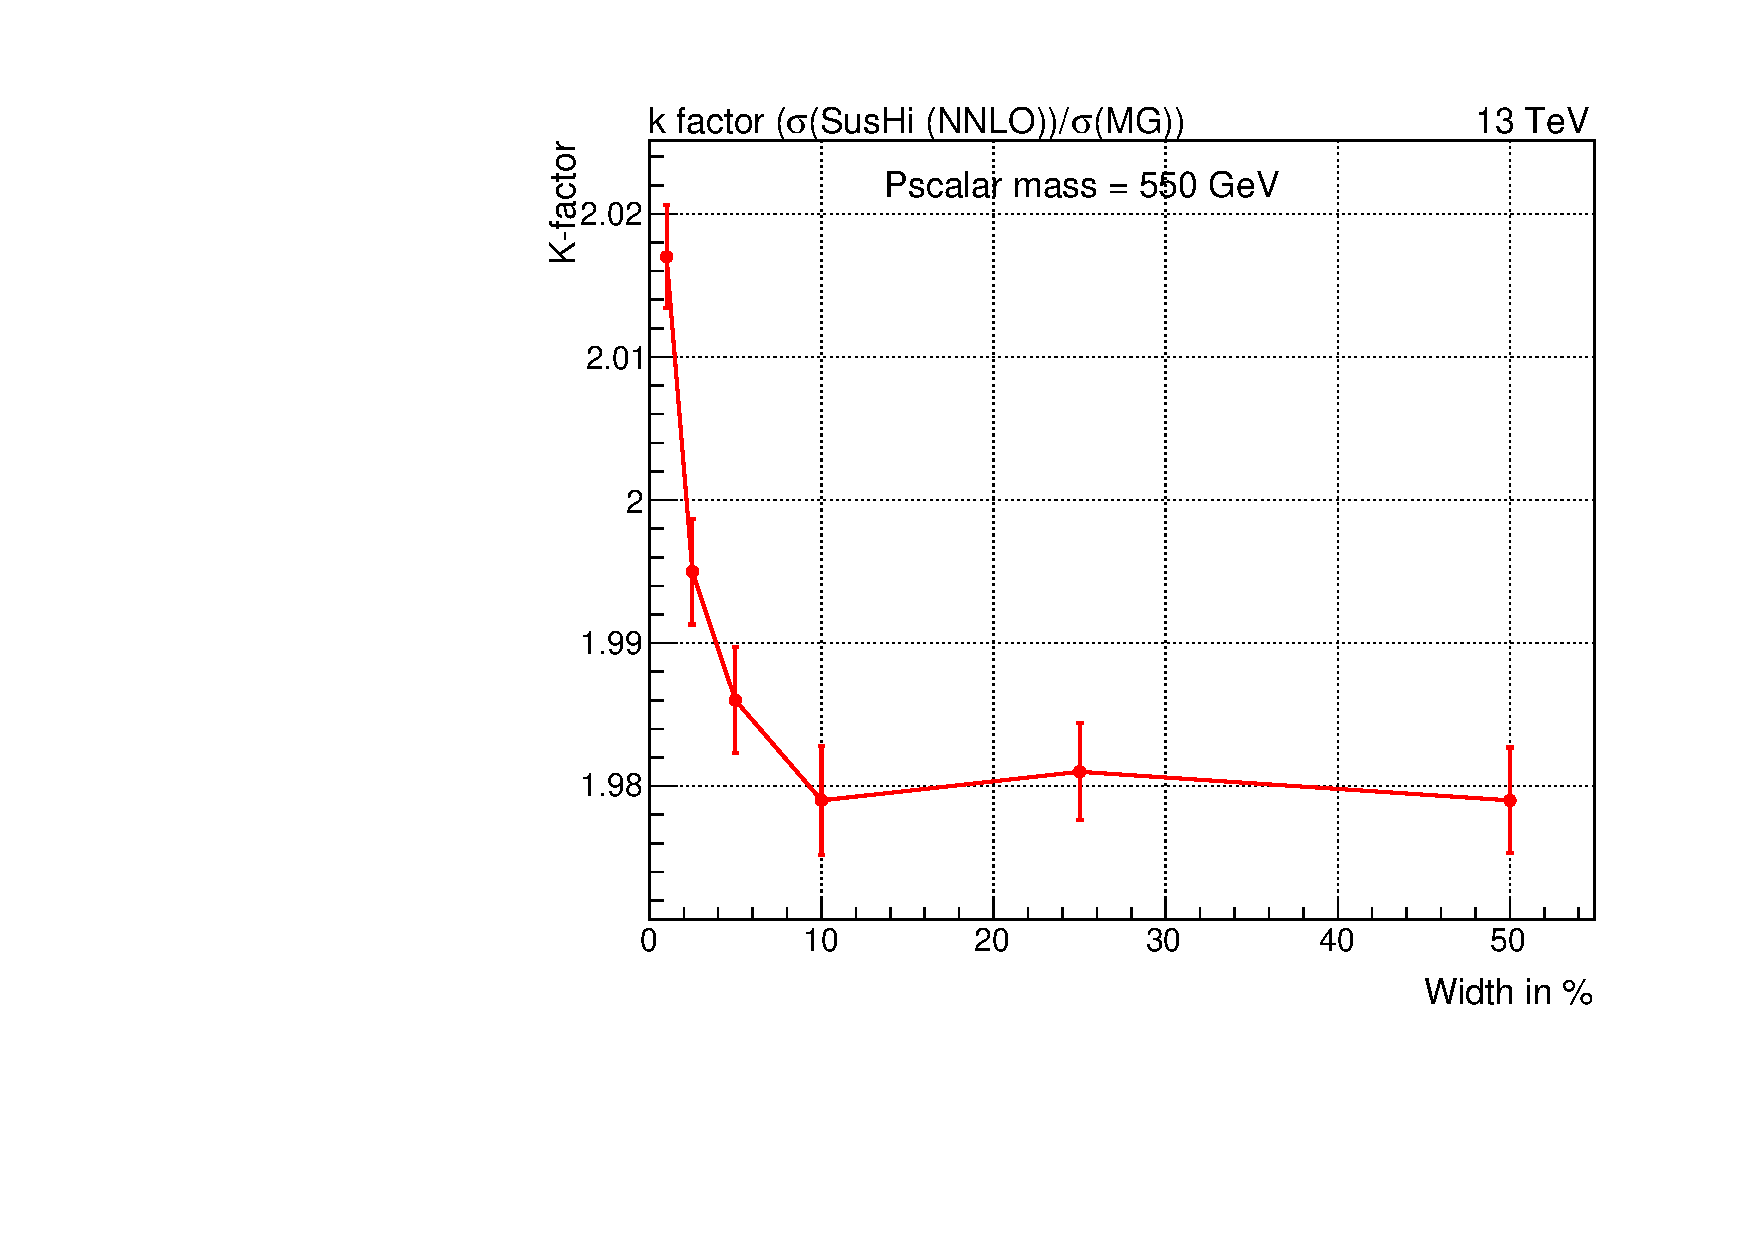
\includegraphics[scale=0.4]{fig/chapt4/k_factor_PScalar_m550_res.pdf}
& \hspace{-0.95cm} 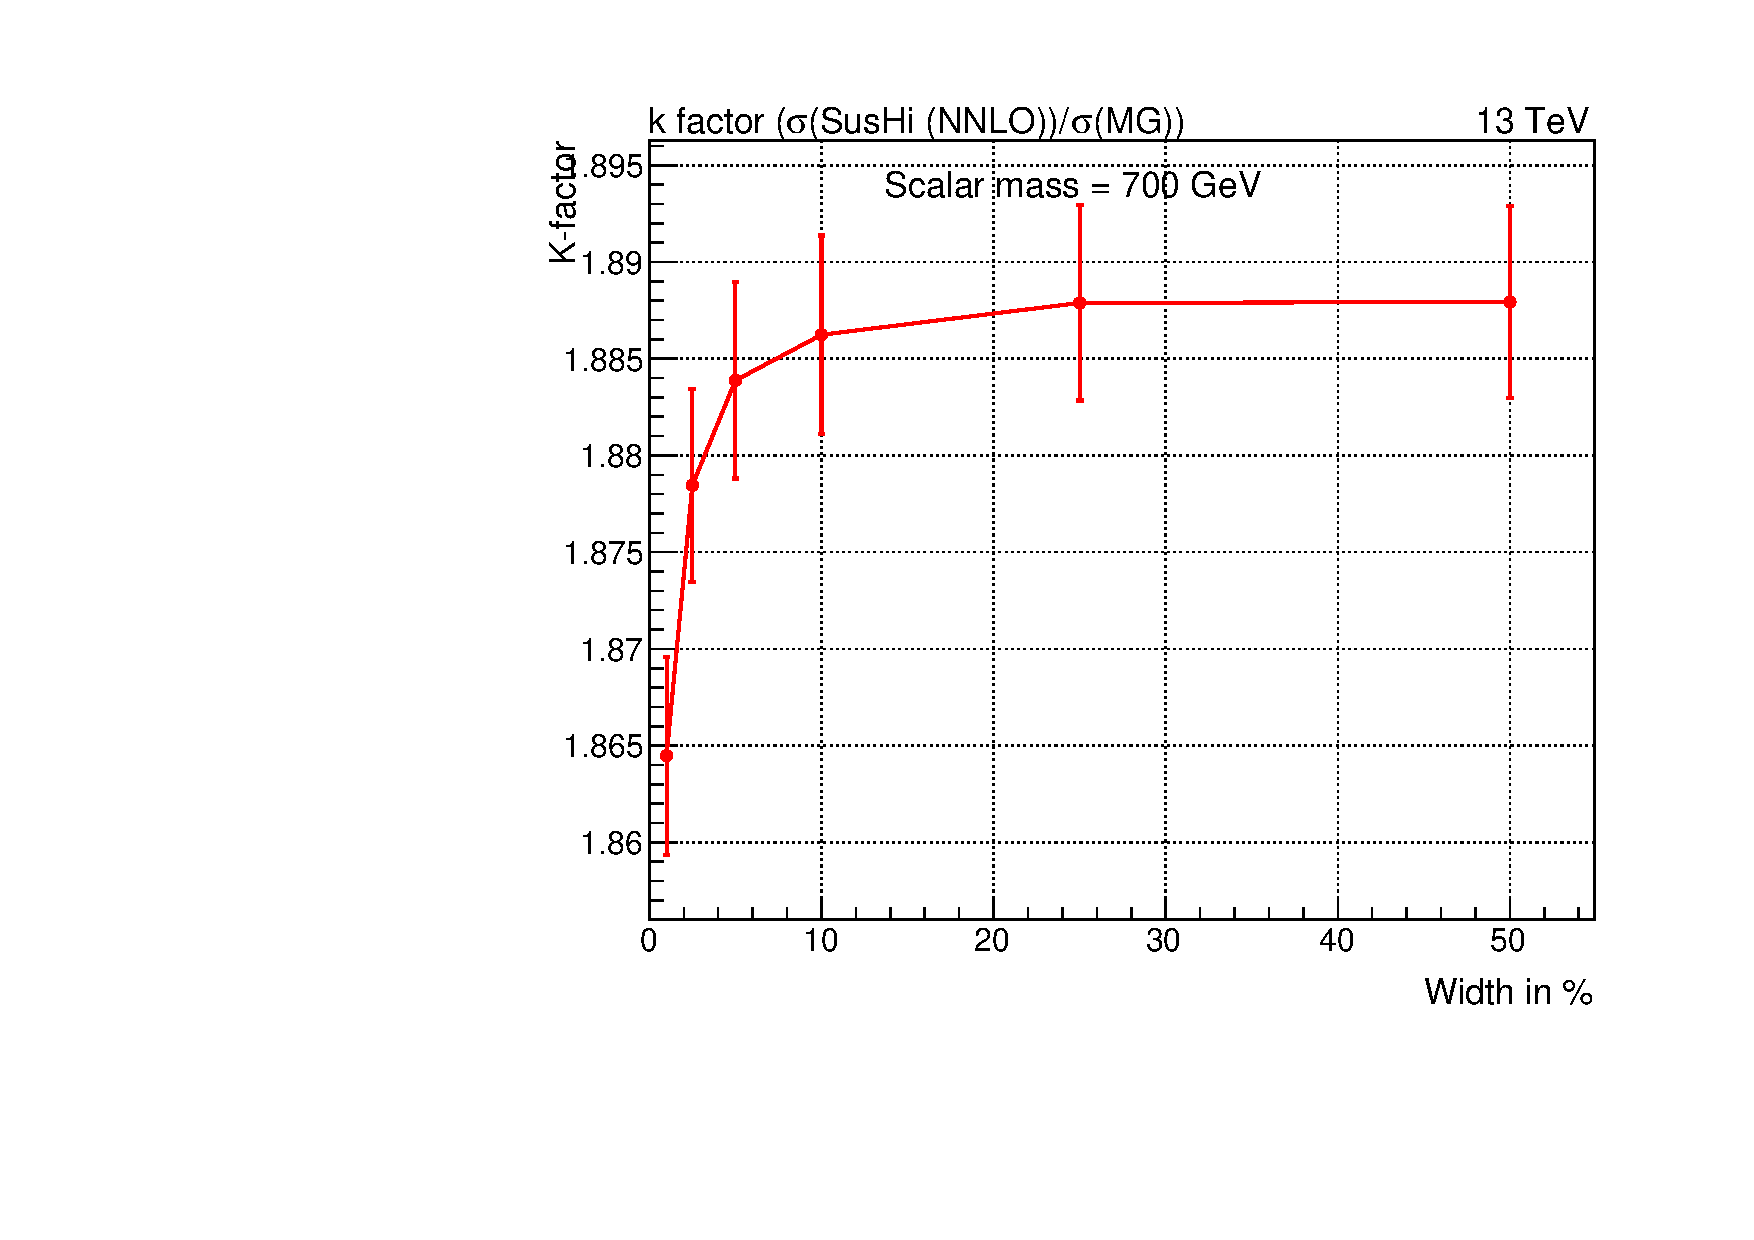
\includegraphics[scale=0.4]{fig/chapt4/k_factor_Scalar_m700_res.pdf}\\
($\mathbf{a}$)\qquad\qquad&($\mathbf{b}$)\qquad\qquad\\ \\
\caption{Typical k-factor for pseudo-scalar mass = 550\,GeV (a) and scalar mass = 700\,GeV (b), obtained from the ratio of $\sigma_{NNLO}$(\textsc{SusHi}) to $\sigma$(MG). Both \textsc{SusHi} and MG LO cross sections are comparable, which leads to the same results if we use $\sigma_{LO}$(\textsc{SusHi}) instead of $\sigma_{LO}$(\textsc{SusHi}). For the whole range of width, the k-factor shows universality, which is easy to apply for other width values \label{fig:k_factor}.}
\end{tabular}
\end{figure}

\subsection{\textsc{Top++}}\label{subsec:top_pp}
The program \textsc{Top++}~\cite{Czakon:top_pp} calculates the total inclusive cross-section for top pairs production in hadronic collisions using two different approaches a) fixed order with NNLO accuracy and b) including soft-gluon resummation in Mellin space with full next-to-next-to-leading logarithmic order (NNLL) accuracy matched through NNLO. \textsc{Top++} is the only publicly available program using soft-gluon resummation for the $t\bar{t}$ inclusive production cross section in hadron colliders.
The \textsc{Top++} program is based on C++ coding in a modular and easy manner with a single configuration file ($\texttt{top++.cfg}$) for user interface. The configuration file consists of simple input parameters such as the type of collider, PDF set, pure fixed order calculation versus one with resummation, mass of top quark, and LO, NLO, and NNLO orders. In this work, we use \textsc{Top++} to calculate the $t\bar{t}$ hadronic cross section up to NNLO accuracy with soft-gluon resummation and LO cross section without soft-gluon resummation. From these two cross sections, the k-factor ($\sigma(NNLO)/\sigma(LO)$) has been calculated for further scaling of interference. The input parameters used for this study (PDF sets) are \textsc{nnpdf30} for NO and NNLO; the top quark mass is 172.5\,GeV, $\mu_{\text{R/F}}$ scale varied as 0.5, 1, and 2.  

  




\clearpage{\pagestyle{empty}\cleardoublepage}
